\chapter{Results}
\label{ch:resu}

\noindent This section presents the quantitative results of our experiments with the methods introduced in \autoref{sec:single-unit-testbench}, \autoref{sec:monolithic-approach}, and \autoref{sec:hybrid-approach}. Here's an outline of our result presentation:

\begin{itemize}

\item In \autoref{sec:single-unit-testbench-results} we present results from the single-agent testbench, utilizing metrics such as \textbdd{episode length}, which represents the survival duration of at least one factory of the learning agent, \textbdd{ice dug}, indicating the amount of ice collected by the unit, and \textbdd{ice transferred}, indicating the amount of dug resource given to the factory. The performance of the algorithms is assessed over 1 million steps, resulting in 125 evaluation phases, each comprising 10 updates, totaling 1,250 model updates. The batch size used is 1,024 over rollouts of size 8,192.

\item In \autoref{sec:monolithic-approach-results} we present results from the monolithic network outlined earlier. We use similar metrics as in the single-unit testbench, but introducing the \textbdd{limitation of training episode lengths from 1,024 to 256} to introduce higher \textbdd{quality data} in our rollout buffers. We also reduced the total training steps from 1 million to 104,200, thus achieving 13 rollout phases, 10 epochs each, achieving 130 model updates with the same batch sizes. We also evaluated our top performer model over 1 million steps to assess its convergence capabilities, meaning keeping alive at least one factory for 1,000 steps (\autoref{fig:mono-dash-1M}).

\item In \autoref{sec:hybrid-approach-results} we showcase the novelty of our research: the results on the hybrid agent control. This approach incorporates trajectory separation, distributed credit assignment, multiple actor and value heads, and a highly scalable feature extractor. We introduce a new metric called \textbdd{average factory alive}, indicating not only the agent's capability to keep one factory alive but multiple factories. We conduct experiments with \textbdd{different trajectory numbers} (\autoref{subsec:modulus-grouping}), including \textbdd{top $N$ unit trajectories}, \textbdd{trajectory groupings} (\autoref{subsec:trajec_reduc}), and \textbdd{interchanging separate trajectories with global rewards and advantages} (\autoref{subsubsec:rewardass}). Additionally, we \textbdd{compare our methods with other works} (\autoref{subsec:comparison}) and present a comprehensive \textbdd{ablation study} (\autoref{subsec:ablation}).

\end{itemize}

\section{Single Unit Testbench}
\label{sec:single-unit-testbench-results}

\noindent For our initial comparison, we focused on environment-related metrics such as \textbdd{episode length}, \textbdd{ice dug}, and \textbdd{ice transferred} by units to determine which algorithm performed best in exploration and resource collection tasks. It's important to note that the results presented in \textcolor{deepblue}{\autoref{tab:single-agent-result-env}} are averages from the best-performing evaluation phase out of $125$ evaluation phases, each consisting of 12 environments.

\bigskip

\begin{table}[htbp]
    \centering
    \begin{tabular}{|c|c|c|c|c|c|}
        \hline
        \textbf{Algorithm Type} & \textbf{Algorithm} & \textbf{Episode Length} & \textbf{Ice Dug} & \textbf{Ice Transferred}\\
        \hline
        \multirow{5}{*}{Policy Gradient Methods} & TRPO  & 582  &  4504  & 4320 \\
        \cline{2-5}
         & A2C & 154 &  136  &  62\\
        \cline{2-5}
         & PPO & 473  & 6814  & 6600 \\
        \cline{2-5}
         & R-P\textbf{}PO  & 612 & 6325  & 5892\\
        \cline{2-5}
         & \textbf{M-PPO}  & \textbf{930} &  \textbf{12780} &  \textbf{12340}\\
        \hline
        \multirow{2}{*}{Value-Based Methods} & DQN & 200  & 256  &  204\\
        \cline{2-5}
         & QR-DQN & 690  &  8112 &  8004 \\
        \hline
        Evolutionary Method & ARS & 154 &  0 &  0\\
        \hline
    \end{tabular}
    \captionsetup{justification=justified, singlelinecheck=false, width=1\linewidth, labelfont=bf} 
    \caption{The table presents environment-related results from the single-unit testbench, emphasizing the top performer among all algorithms. \textbdd{M-PPO emerged as the standout performer} among policy gradient methods (\autoref{sec:Policy-Gradient-Methods}), showcasing superior performance attributed to its action masking method. Additionally, R-PPO demonstrated improved performance over standard PPO due to its recurrent nature. Surprisingly, the second-best performing algorithm was a value-based method (\autoref{subsec:value-based-methods}), \textbdd{QR-DQN}, which achieved an average episode length of 690 during its best evaluation phase. QR-DQN also exhibited significant enhancements compared to its standard variation without quantization techniques.}
    \label{tab:single-agent-result-env}
\end{table}

\begin{figure}[htbp]
    \centering
        \centering
        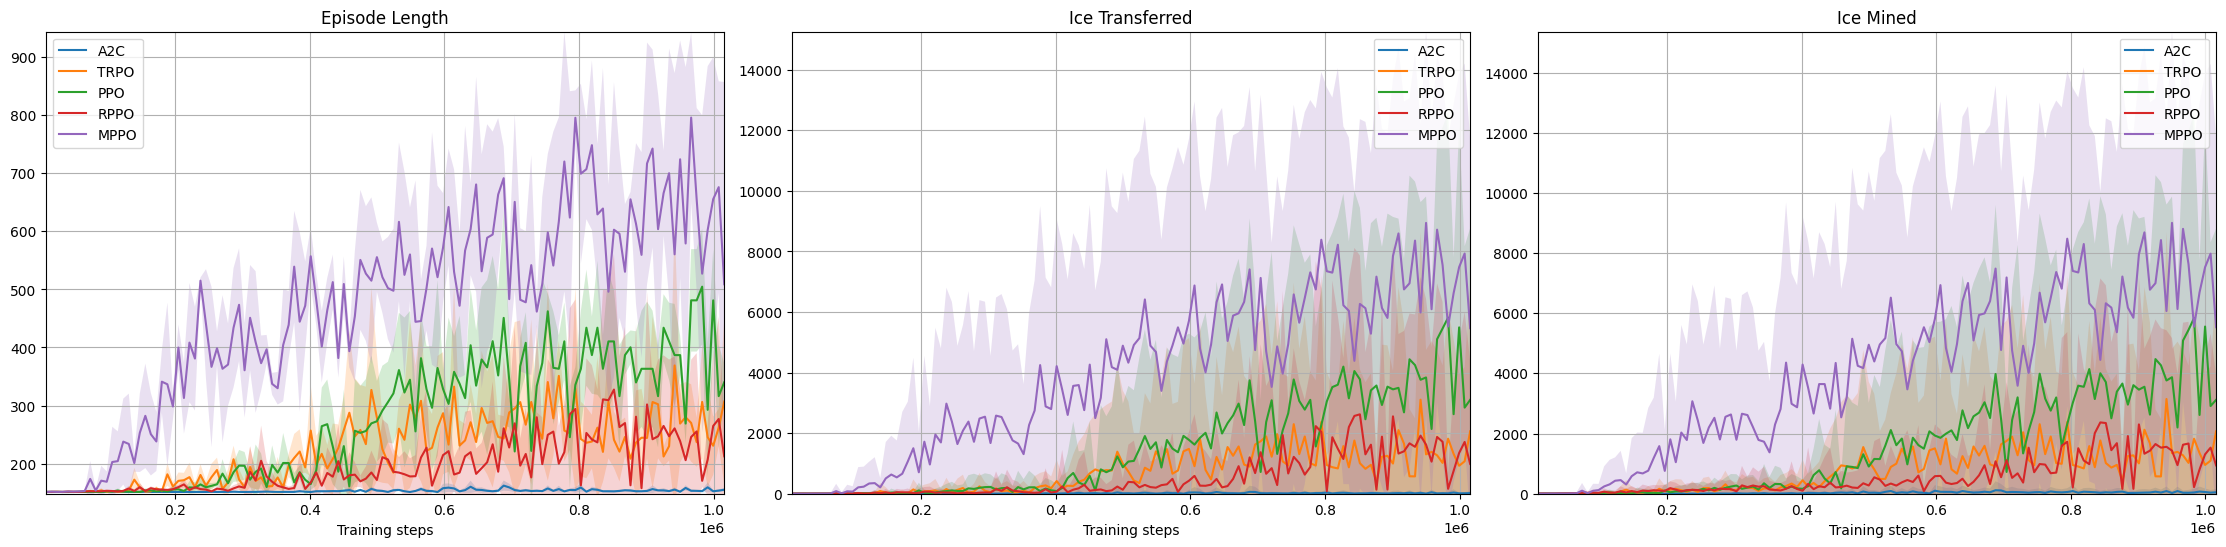
\includegraphics[width=\linewidth]{images/results_singleunit/policy_gradient_single_unit.png}
        \captionsetup{justification=justified, singlelinecheck=false, width=1\linewidth, labelfont=bf} 
        \caption{The three plots depict averages from all three trials of all policy gradient methods alongside their respective evaluation phases, illustrating the average \textbdd{episode lengths}, average \textbdd{ice transferred}, and \textbdd{ice dug}. The data indicates that nearly all policies learned to transfer the collected resource of the unit after digging, as evidenced by the clear similarity between the ice transferred and ice dug plots. Moreover, the images highlight the effectiveness of the invalid action masking technique in M-PPO, which accelerates the learning progress. This is evident from the \textbdd{sharp increase in averages after 204,800 steps}, while maintaining stable updates to the policy.}
        \label{fig:policy_gradient_single_unit}
\end{figure}

\noindent Examining the policy gradient algorithms in \autoref{fig:policy_gradient_single_unit}, we observe that \textbdd{PPO and M-PPO exhibit superior performance} compared to other policy gradient methods in terms of averages. Notably, R-PPO demonstrates higher peaks compared to PPO. Additionally, the plots reveal that certain algorithms, such as \textbdd{A2C, exhibit stagnation with notably low performance}. \textbdd{TRPO} also appears to \textbdd{remain divergent} in a local optimum throughout the evaluations, likely due to its larger updates compared to PPO.

\bigskip

\begin{figure}[htbp]
    \centering
        \centering
        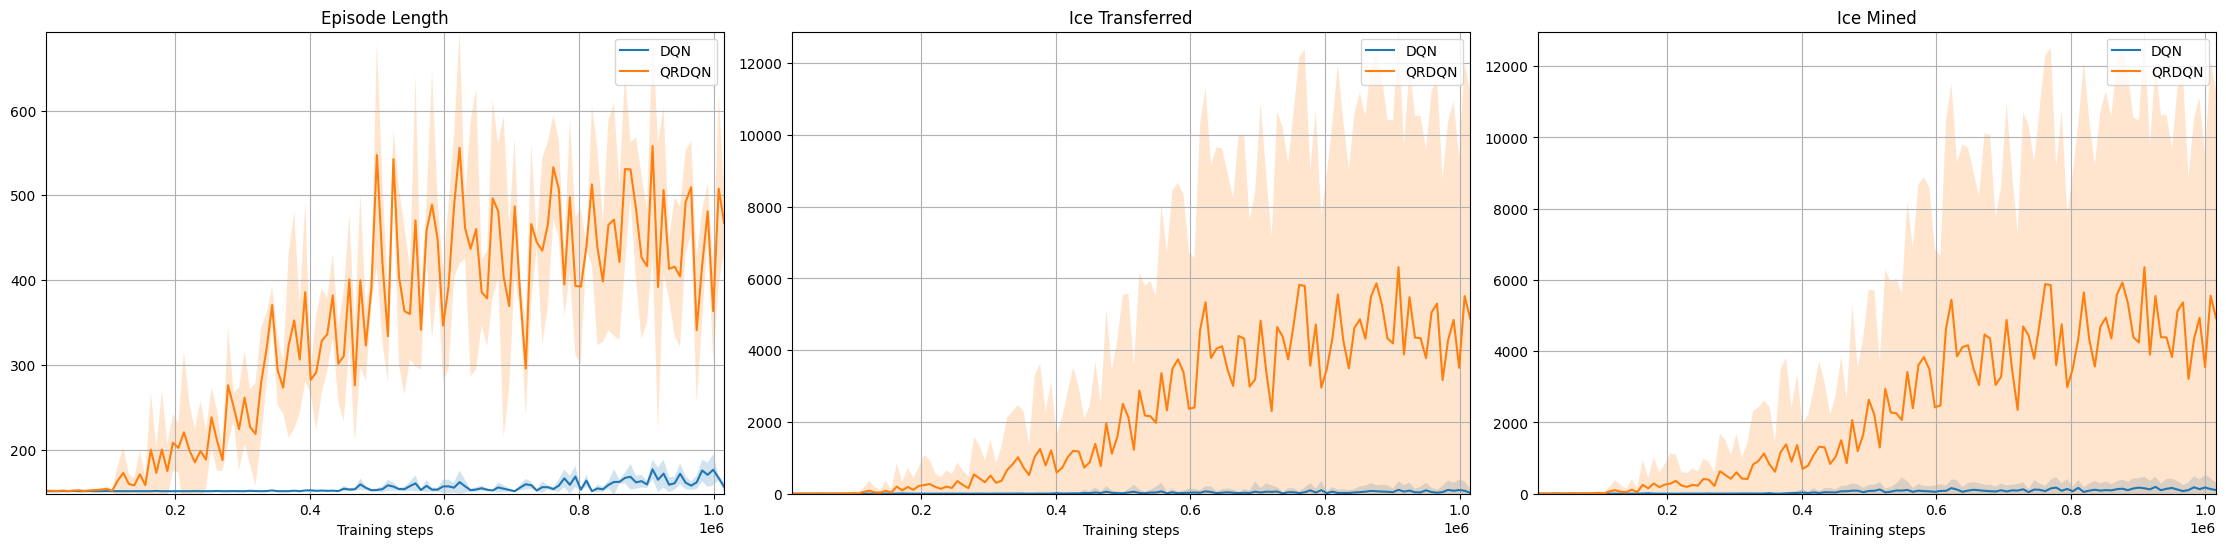
\includegraphics[width=\linewidth]{images/results_singleunit/value_based_single_unit.png}
        \captionsetup{justification=justified, singlelinecheck=false, width=1\linewidth, labelfont=bf} 
        \caption{The three plots display averages from all three trials of all value-based methods, showcasing their performance across various evaluation phases. They illustrate the average \textbdd{episode lengths}, average \textbdd{ice transferred}, and \textbdd{ice dug}. The results highlight a noticeable difference in performance between the two algorithms, with QR-DQN demonstrating significant improvements attributed to its quantization technique.}
        \label{fig:value_based_single_unit}
\end{figure}

\noindent The results depicted in \autoref{fig:value_based_single_unit} clearly \textbdd{favor QR-DQN} for our task. However, it's important to address a significant difference in performance between these two algorithms. QR-DQN utilizes 200 quantiles for its Q value estimates for every state-action pair, leading to a \textbdd{200-fold increase in the output size of the Q-network} compared to its DQN counterpart. This substantial increase in network complexity results in a significant degradation in training performance, with QR-DQN achieving a \textbdd{step-per-second (SPS)} processing speed of 10 compared to DQN's 832. In this context, \textbdd{SPS} refers to the rate at which the algorithm processes steps or actions within the environment per unit of time, measured in seconds. Steps per second were calculated during evaluation phases, including both backward and forward passes during model updates, where a higher SPS indicates better performance.

\begin{figure}[htbp]
    \centering
        \centering
        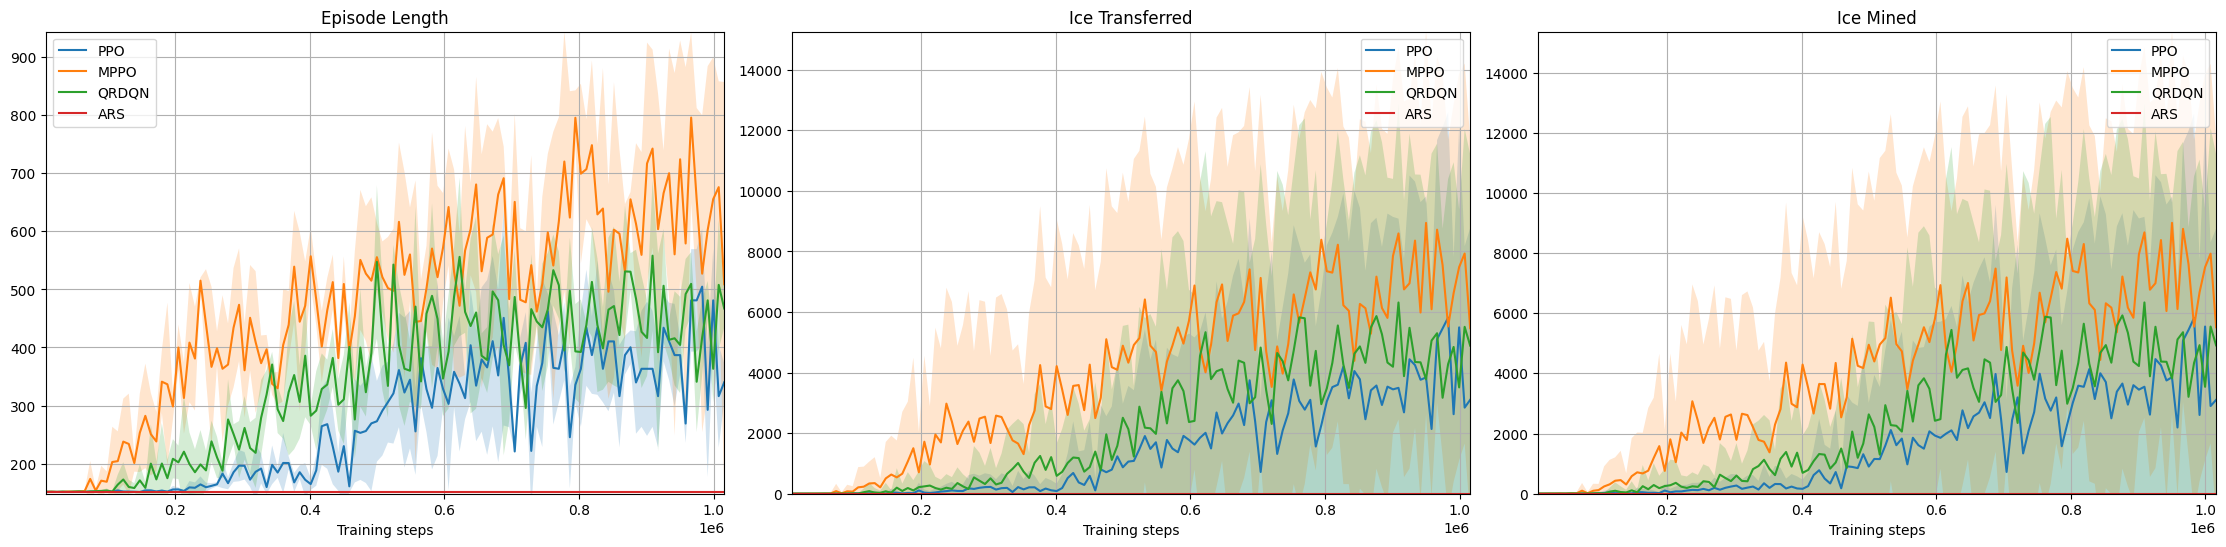
\includegraphics[width=\linewidth]{images/results_singleunit/total_single_unit.png}
        \captionsetup{justification=justified, singlelinecheck=false, width=1\linewidth, labelfont=bf} 
        \caption{In a comprehensive final comparison of the top-performing policy gradient algorithms (PPO, M-PPO), the value-based algorithm (QR-DQN), and the sole neuro-evolution algorithm (ARS).}
        \label{fig:total_single_unit}
\end{figure}

\noindent The data in \textcolor{deepblue}{\autoref{fig:total_single_unit}} validates a key assumption: \textbdd{masking out invalid actions in the environment}, thereby limiting the exploration space, proves \textbdd{advantageous in early training}. This approach accelerates learning by preventing illegal moves. The ongoing cost of recalculating masks in later training stages yields diminishing returns, as the model naturally learns to avoid meaningless actions over time. Nonetheless, this trade-off is highly favorable, as the early acceleration is essential to prevent the agent from getting stuck in local optima, and the minor decrease in training speed during later phases is acceptable. \textbdd{ARS falls short of expectations} in more complex environments characterized by large action spaces and sparse rewards. The algorithm struggles to navigate such environments effectively, particularly because rubble must be destroyed for ice to be mined. Without heavy reward shaping, it is highly improbable for a random search algorithm like ARS to consistently identify the correct rubble location and continue digging until the rubble is destroyed, leading to ice mining and reward collection.

\bigskip

\noindent Based on the observed results, we decided to \textbdd{transition from the single-unit setting to a multi-agent environment} using the \textbdd{M-PPO algorithm}. This decision was influenced by M-PPO's stable learning behavior facilitated by clipping techniques and its capability to converge to an optimal policy by masking out invalid actions within the environment.


\section{Monolithic Approach}
\label{sec:monolithic-approach-results}

\noindent In this section, we analyze various results of our monolithic approach (\autoref{sec:monolithic-approach}), focusing on its \textbdd{potential and limitations} in the Lux AI environment. We compare different network architectures, including a U-net type neural network with two distinct bottleneck techniques (\autoref{fig:Bottlenecks}) and another architecture that maintains the original size of the input observation (\autoref{sec:monolithic-network}). The \textbdd{BottleNet} architecture achieves the creation of a \textbdd{class system} within the network, allowing it to produce a segmentation map where each pixel corresponds to a specific action that a unit can take, such as digging or recharging. In contrast, the DashNet architecture maintains the original height and width dimensions, effectively mapping each piece of information provided by a pixel to an action. This mapping is achieved while also considering other parts of the network through convolution operations.

\bigskip

\noindent The addition of \textbdd{squeeze-and-excitation layers} (\autoref{subsec:se}) in our architecture played a critical role in improving our mapping and classification objectives. Initially, when these layers were omitted, we observed a notable decrease in model performance. Squeeze-and-excitation layers dynamically modulate the importance of feature maps, thereby increasing their contribution to accurate mapping from observation to input. Notably, the feature channel representing ice resources on the map exhibited significant influence on the digging action when combined with the unit map.

\bigskip

\noindent We introduced a \textbdd{novel masking method} designed to align with the principles of Proximal Policy Optimization, aiming to constrain the magnitude of updates through its clipping mechanism. This method involved invalidating all actions for map spaces devoid of entities, except for the no-operation action, thereby establishing \textbdd{determinism in empty pixels}. This deterministic approach introduced minimal noise to updates, as updates primarily occurred in regions occupied by entities. Specifically, on a $48\times48$ map typically involving $30$ entities, with approximately $4$ factories and $26$ units, out of $2,304$ pixels, updates were concentrated in areas where entities were present. Consequently, our masking policy utilized small updates, mitigating the risk of policy collapse or entrapment in local optima. During training, we consistently observed improvements in performance without encountering any instabilities. Throughout updates, \textbdd{KL divergence remained minimal} with respect to the policy, typically falling within the expected range for PPO, between 0 and 1. This suggests that the probability of a certain action doubled at most, indicating that $P$ was approximately twice as likely as $Q$ for that specific outcome, measured on a binary logarithmic scale. Moreover, we observed a minimal clipping fraction for gradient updates, typically ranging between 0.1 and 0.2, indicating that the \textbdd{model did not attempt overly aggressive updates}.

\subsection{DashNet vs BottleNet}

\begin{figure}[htbp]
    \centering
    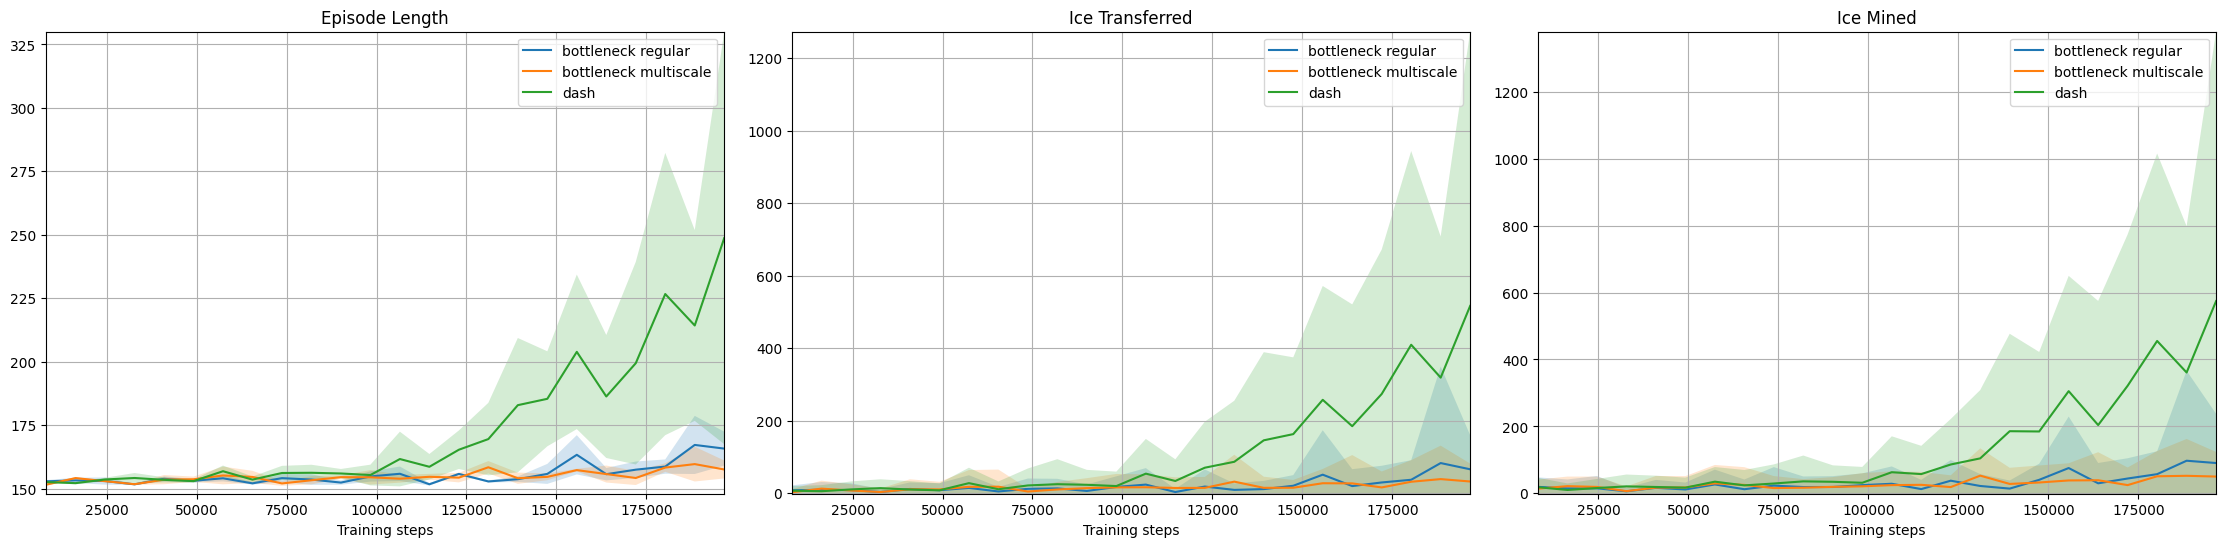
\includegraphics[width=1\linewidth]{images/results_monolithic/mono_results.png}
    \captionsetup{justification=justified, singlelinecheck=false, width=1\linewidth, labelfont=bf} 
    \caption[]{The plot compares the performance of the monolithic approach in terms of evaluation metrics, including the length of episodes, ice transferred by units, and ice mined. The data clearly demonstrates the superiority of DashNet over both BottleNets. DashNet shows improvement across all aspects, achieving higher training speeds, similar fluctuations, stable learning behavior, and consistent enhancement, particularly notable after 81,920 steps.}
    \label{fig:mono_results}
\end{figure}


\noindent \autoref{fig:mono_results} presents the performance of both algorithms based on evaluation metrics such as average \textbdd{episode length, ice dug, and ice transferred}. The episode length metric serves the same purpose as in the single-unit testbench (\autoref{sec:single-unit-testbench-results}), evaluating the ability of the global policy to sustain factories. Ice dug and ice transferred metrics are employed for \textbdd{alignment checking}, as these actions were positively rewarded in the environment. The results represent data from three trials, trained from scratch up to 204,800 steps. This extended training duration was necessary due to SB3's lack of self-play support during development, doubling our initial target of 102,400 steps. Thus, we provided the model with the same amount of data, albeit from the same on-policy perspective. Batch sizes and rollout steps were also doubled to align with our 102,400-step target. While all algorithms showed an increasing trend in performance, the \textbdd{U-net architecture fell behind after 81,920 steps}. This suggests that downsizing the observation space to a small bottleneck size and attempting to reconstruct a class map through on-policy optimization results in smaller updates, leading to slower learning compared to maintaining the original input size and finding a correct same-size mapping in neural network space.

\begin{table}[h!]
    \centering
    \begin{tabular}{|c|c|}
        \hline
        \textbf{Algorithm} & \textbf{Longest Evaluation Episode} \\
        \hline
        Simple BottleNet     & 178 steps \\
        Multiscale BottleNet & 167 steps \\
        \textbf{DashNet}    & \textbf{325 steps} \\
        \hline
    \end{tabular}
    \captionsetup{justification=justified, singlelinecheck=false, width=1\linewidth, labelfont=bf} 
    \captionof{table}{The table displays the longest evaluation episode, indicating which episode out of the total 274 (derived from 12 episodes across 25 evaluation phases) had the longest surviving factory (higher is better).}
    \label{tab:mono-results-table}
\end{table}

\subsection{DashNet Convergence Study}

\noindent As for a final study, we aimed to assess the convergence potential of the superior DashNet model by \textbdd{extending its training duration} to 1 million steps, a fivefold increase compared to previous trials. We also explored alternative configurations, such as removing normalization layers and residual blocks from the network, but found that they led to poor performance. Additionally, extensive ablation studies were conducted as part of the hybrid method, detailed in \autoref{subsec:ablation}, to examine the significance of regularization techniques, network depth, and factory placement and bidding heuristics.


\begin{figure}[htbp]
    \centering
    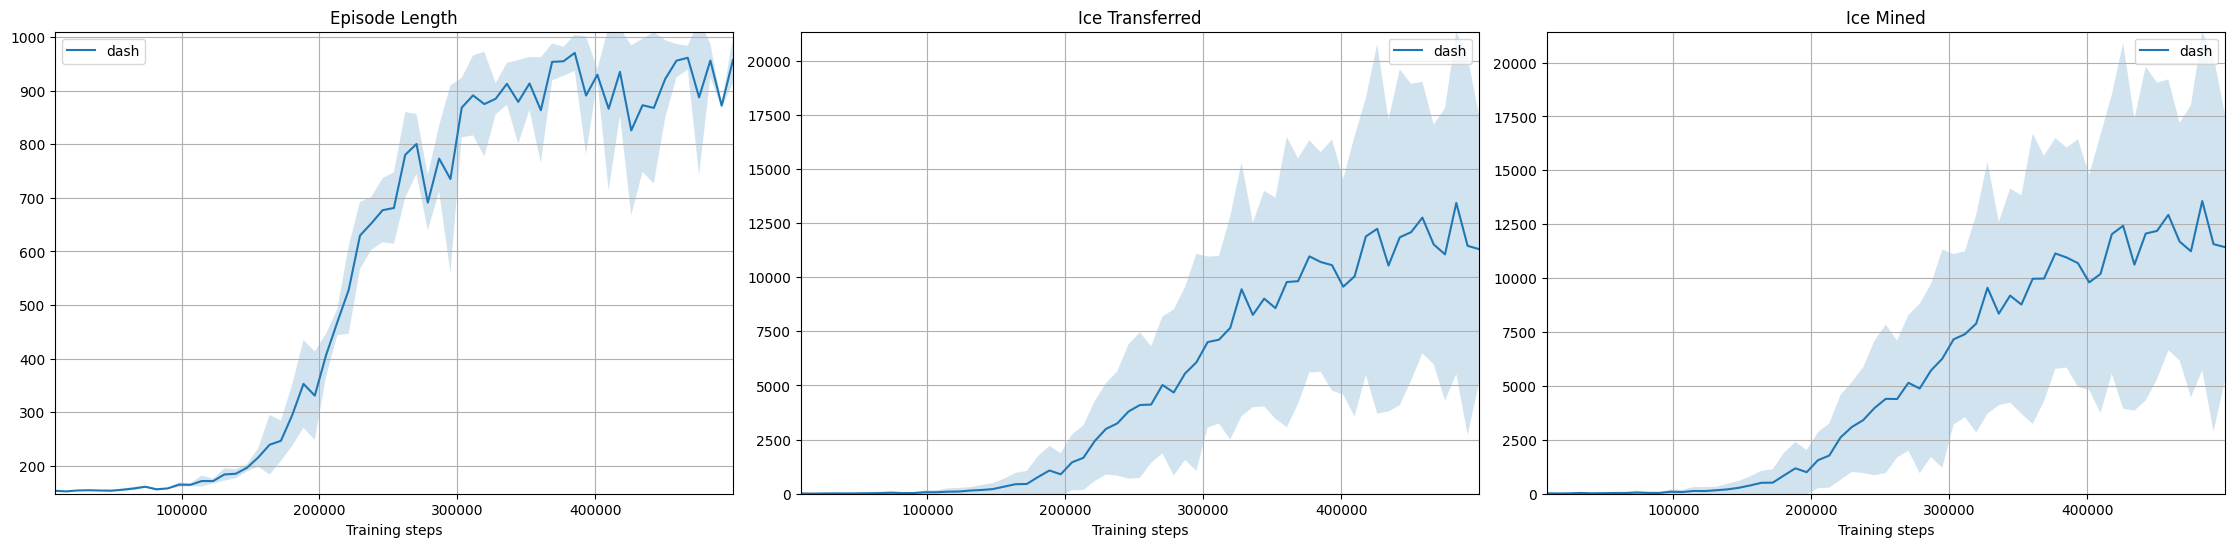
\includegraphics[width=1\linewidth]{images/results_monolithic/dash_1m.png}
    \captionsetup{justification=justified, singlelinecheck=false, width=1\linewidth, labelfont=bf} 
    \caption[]{The image illustrates the results obtained from the \textbdd{DashNet architecture}, averaged over three trial runs, with each trained until 507,904 training steps. The plots indicate that the algorithm converges around an average episode length of 1000, exhibiting minor fluctuations attributed to sparse updates resulting from architectural specifications.}
    \label{fig:mono-dash-1M}
\end{figure}

\bigskip

\noindent \autoref{fig:mono-dash-1M} illustrates the model's progression beyond the initial exploration phase, demonstrating a \textbdd{snowball effect} in algorithm performance as it refines its policy. While the model achieved an average of \textbdd{1024 steps in $\mathbf{95\%}$ of the evaluation environments} after 507,904 training steps, this progress was achieved at a significant cost and slow pace. The combination of the monolithic approach exhibited great potential; however, there are numerous optimization opportunities for further improvement, despite the semi-paradoxical nature of its learning dynamics. These optimization opportunities are addressed in the hybrid approach (\autoref{sec:hybrid-approach-results}).

\bigskip

\noindent Consistent updates led to the achievement of a \textbdd{convergent policy}; however, efficiency remains a concern. Given our monolithic approach, especially during initial training stages, \textbdd{suboptimal actions are often reinforced}. This is because only a minority of entities exhibit positive behavior, while the majority engage in non-beneficial actions. To address this, the model requires active engagement from at least half of the entities, plus one, in positive actions, while the remaining entities may persist with suboptimal actions, thereby influencing the overall learning dynamics of the model.

\bigskip

\subsection{Against the Odds}

\noindent In the following, we analyze a hypothetical scenario, in which we train a model from scratch and consider a map with 30 entities. These entities include 4 factories, 4 heavy units, and 22 light units. In this scenario, we can hypothesize the following: Factory actions do not yield immediate rewards directly to the model. However, through the production of units, positive actions are indirectly initiated in all instances. When a factory depletes its resources, its sole feasible action is \textbdd{no operation}, which inherently benefits the model as it facilitates resource conservation. Thus, \textbdd{factories consistently contribute positively to the model's performance}.

\bigskip

\noindent When considering units, our analysis must be split to address heavy units separately from light units. For heavy units, achieving a rewarding action is exceedingly unlikely. A hypothetical assessment may be outlined as follows: Typically, units have access to approximately 5 possible actions on average, due to the masking of invalid actions. However, in most cases, only one action results in a rewarding outcome. Moreover, the likelihood of achieving a reward is further diminished, as it necessitates a sequence of optimal actions. Heavy units are generally capable of achieving this within 5 steps, resulting in an individual \textbdd{heavy unit having a probability of only $\mathbf{4\%}$ to attain a possible reward}. To ascertain the probability of at least 3 units achieving this, we resort to the binomial distribution (\cite{enwiki:1223310929}). The probability mass function of a binomial distribution is given by:

\begin{equation}
P(X = k) = \binom{n}{k} p^k (1-p)^{n-k},
\label{eq:binomial}
\end{equation}

where

\begin{itemize}[itemsep=4pt, parsep=0pt]
    \item \( n \) is the number of trials (4 - heavy, 22 - light),
    \item \( k \) is the number of successful trials (3 - heavy, 13 - light),
    \item \( p \) is the probability of success on a single trial \( \left( (\frac{1}{5})^5 \text{ - heavy},  (\frac{1}{5})^{10}  \text{ - light} \right) \).
\end{itemize}



\noindent For heavy units, this yields a probability of approximately $2.45 \times 10^{-4}$. Conversely, for light units, with a much larger population, where a rewarding action occurs on average every 10 steps, \textbdd{the probability is even smaller}, falling within the range of $1 \times 10^{-61}$. To appropriately weigh these probabilities, it's important to consider that heavy units offer 10 times more opportunities for rewards in terms of magnitude in a single step. However, even after adjusting for this factor, the final probability remains \textbdd{exceedingly small and negligible}, akin to winning the lottery six times in a row or achieving a perfect shuffle of a 52-card deck. It's essential to note that these calculations are approximate and valid only prior to the first update to the model, as action probabilities follow a uniform distribution. 

\bigskip

\noindent The purpose of the above calculations was to provide an \textbdd{order of magnitude} type estimation (rather than precise numerical calculations), in order to demonstrate the unlikeliness of the model achieving a significant reward, and thus a substantial update, at the beginning of the training phase. Naturally, as the model learns better policies, these probabilities increase, leading to higher chances of learning the optimal action for a given state. Given the sparsity of the monolithic method and the myriad optimization possibilities it presents, we decided to focus our efforts on evaluating our novel proposal of trajectory separation and a hybrid approach for PPO.

\bigskip

\section{Hybrid Approach}
\label{sec:hybrid-approach-results}

\noindent In this section, our primary focus will be on showcasing the effectiveness of our technique called \textbdd{trajectory separation} (\autoref{subsec:grouping}) to demonstrate its potential for improving the hybrid architecture (\autoref{sec:hybrid-approach}). In addition, we will explore potential enhancements and limitations of the method, including examining the components of trajectory separation to determine the specific factors that contribute to the improvement of performance. We will also conduct a comparative analysis between the trajectory-separated hybrid, \textbdd{pixel-to-pixel} architecture (\autoref{par:pixel-to-pixel}) and existing solutions for the Lux AI competition. At the end of the section, an ablation study will be carried out, analyzing the methods in addition to trajectory separation.

\bigskip

\noindent In the subsequent configurations, factories, and units will be organized into distinct groups, each with aggregated outputs and trajectories. Groups can exhibit various characteristics, from global groups encompassing all entities of a specific type to individual groups in which each entity functions as its own separate group. In this study, we illustrate the significance of distinct trajectories within a multi-agent setting and investigate various approaches for distributing rewards among the agents. All of the experiments shared a common training objective, which was to train the units to keep the factories alive until the end of the game, spanning 1,000 steps. In the following experiments, we will employ the metrics specified in \autoref{sec:hybrid-metrics}. These metrics include the length of an episode, the aggregate amount of ice transferred to factories within a given episode, and the count of operational factories at each environment step, normalized by the maximum episode duration.

\bigskip

\noindent The experiments consist of three separate runs, each utilizing different seeds and running for a total of 102,400 steps (25 training cycles with a 4,096-step batch size). We felt the difference between variants could be sufficiently highlighted in this step range. Contrary to the \textbdd{single-unit} test bench (\autoref{sec:single-unit-testbench-results}) and the \textbdd{monolithic approach} test (\autoref{sec:monolithic-approach-results}), in this scenario, \textbdd{both players are active} and performing actions simultaneously. The \textbdd{same model}, as detailed in \autoref{sec:hybrid-network-architecture}, was used for both players and was trained on their collective trajectories. Following each training cycle, we ran an evaluation of the model by executing 12 distinct environments until the conclusion of the matches. These environments were seeded differently for each of the three runs. The evaluation process yielded 36 data points per training cycle for environment-specific metrics, specifically the metric of \textttdb{Episode Length}. Additionally, by considering each player separately, there were 72 data points for player-specific metrics, including \textttdb{Ice Transferred} and \textttdb{Average Factory Alive}. The lines on the charts visually represent the metrics' means, while the shaded area shows the standard deviation. In addition to the charts, tables are included to make comparisons easier. The columns \textttdb{Final Ice Transferred} and \textttdb{Final Episode Length} refer to the metrics collected at the last evaluation of the model. The mean value is presented, along with the standard deviation in brackets. The \textttdb{X\% of Episodes Finished by} metrics measure how long it took for the agents to learn how to keep the factories alive until the end of the game in terms of environment steps. The percentage indicates the ratio of evaluation environments that resulted in a finished episode, which is an episode where at least one factory survived from both players until 1,000 steps.

\subsection{Trajectory Separation} \label{sec:trajectory-separation}

\subsubsection{Global Trajectory vs Separated Trajectories}

\noindent An initial experiment was done to see what effect \textbdd{separated trajectories} (\autoref{subsec:grouping}) had on how fast the agents learned. As the control group, we implemented a variant that closely resembles the original pixel-to-pixel method (\cite{chen2023emergent}) by utilizing a single \textbdd{global group} (\textttdb{"single global trajectory"}), resulting in a centralized architecture. To evaluate our more decentralized approach, we experimented with various group configurations. These configurations included the formation of distinct \textbdd{global groups} for each entity type (\textttdb{"global factories, global units"}), the creation of a single global group for one entity type while maintaining individual groups for the other (\textttdb{"global factories, separate units"}, \textttdb{"separate factories, global units"}), and the establishment of \textbdd{individual groups} for each entity (\textttdb{"separate trajectories for all entities"}). As demonstrated in \autoref{fig:hybrid_results/trajectory_separation/combined} and \autoref{tab:hybrid_results/trajectory_separation/combined}, the variants with separated trajectories perform much better compared to the global trajectory variants. The most notable improvement is the \textbdd{rate of convergence}, which resulted in the model learning to keep the factories alive until the end of the game by around the 50,000th step, which the fully global variant could not achieve at all. Upon arriving at this significant milestone, the agents continued to improve their strategies further, leading to an average transfer of more than 40,000 ice to factories throughout the 1,000 steps in an episode. The value is 13 times greater than the achievement of the global trajectory variant. The accomplishment was reached by acquiring the skill to transfer ice to all of the factories rather than solely to one, which would have been sufficient to reach the maximum episode length. We can see this by the \textbdd{average factory alive} metric, which continues to rise even after the \textbdd{episode length} levels off at the maximum possible value. The new technique also reduced the \textbdd{frequent fluctuations} of the model's performance, which hinted at unlearning the progress made by the previous steps. We suspect this was the cause of destructive behavior reinforcement, which our method avoids since agents are only rewarded for their actual work (explained in \autoref{subsec:methodcomp}). The findings of the experiment indicate that utilizing separate trajectories can offer a notable benefit to the agents' training process.

\begin{figure}[htbp]
    \centering
    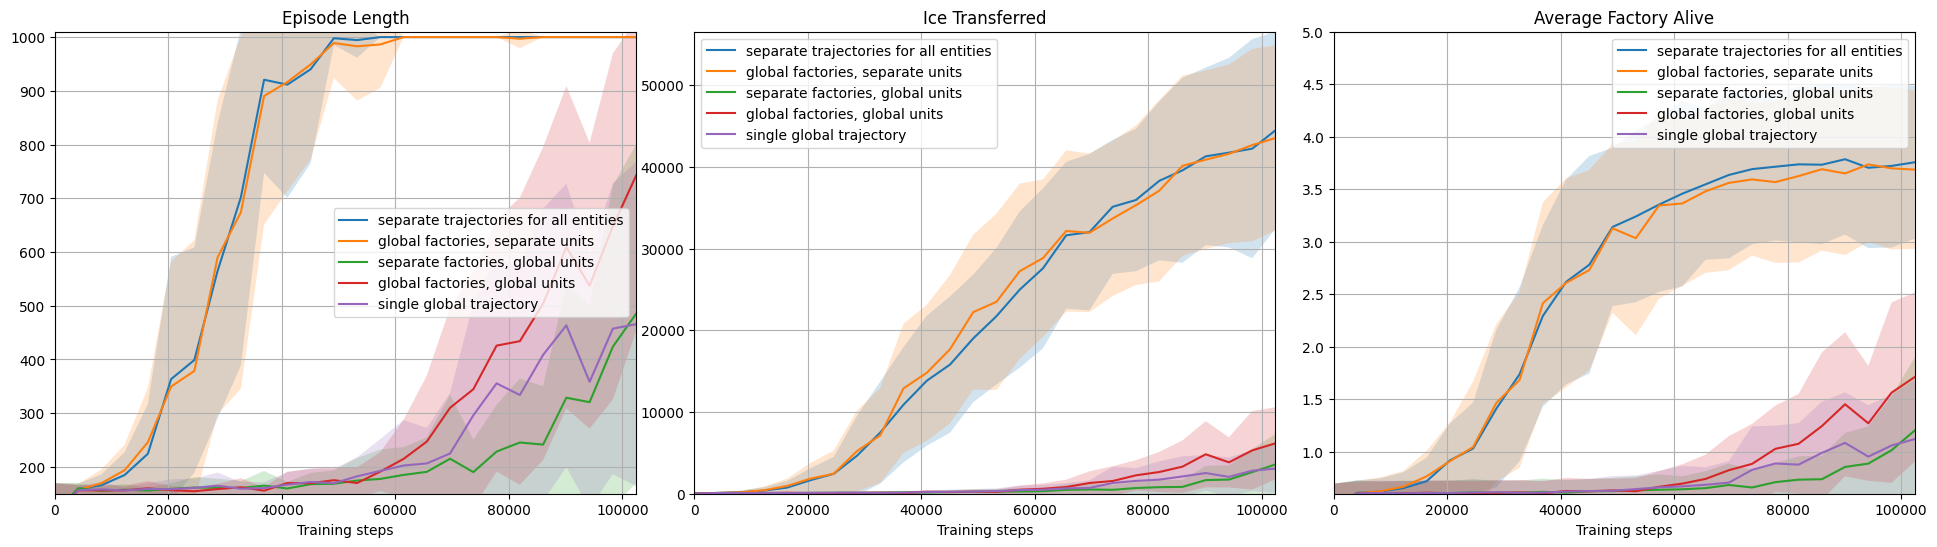
\includegraphics[width=0.95\linewidth]{images/results_hybrid/trajectory_separation/combined.png}
    \captionsetup{justification=justified, singlelinecheck=false, width=1\linewidth, labelfont=bf} 
    \caption[]{Plot comparing the usage of trajectory separation and global trajectories in terms of the length of the episodes, ice transferred by units, and number of active factories. The data presented in the figure indicates a clear improvement in all metrics thanks to the utilization of trajectory separation. In addition to faster convergence, the variants with separated trajectories exhibit reduced fluctuations in performance, thereby leading to more efficient training.}
    \label{fig:hybrid_results/trajectory_separation/combined}
\end{figure}

\begin{table}[ht]
    \footnotesize
    \renewcommand{\arraystretch}{1.2}%
    \begin{tabularx}{\textwidth}{|X|C{2.3cm}|C{2.3cm}|C{2.0cm}|C{2.0cm}|}
        \hline
\multicolumn{1}{|Y|}{\textbf{Group Name}} & \textbf{Final Ice Transferred} & \textbf{Final Episode Length} & \textbf{10\% of Episodes Finished by} & \textbf{95\% of Episodes Finished by} \\
        \hline
separate trajectories for all entities & \textbf{44,472 (12,065)} & \textbf{1,000 (0)} & \textbf{28,672 steps} & \textbf{49,152 steps} \\
global factories, separate units & 43,528 (11,327) & \textbf{1,000 (0)} & \textbf{28,672 steps} & \textbf{49,152 steps} \\
separate factories, global units & 3,573 (3,753) & 485 (315) & 98,304 steps & - \\
global factories, global units & 6,162 (4,413) & 742 (290) & 81,920 steps & - \\
single global trajectory & 3,066 (2,996) & 466 (302) & 102,400 steps & - \\
        \hline
    \end{tabularx}
    \medskip
    \captionsetup{justification=justified, singlelinecheck=false, width=1\linewidth, labelfont=bf} 
    \caption{Table comparing the usage of trajectory separation and global trajectories. The metrics featured include the amount of ice transferred by units and the length of the episodes in the evaluation phase following the last training cycle. The table also contains the observed environment steps needed until the model reaches the maximum episode length in the specified percentage of evaluation environments. The variant with completely separate trajectories was able to provide the factories with 13 times more ice after the training and has managed to reach the maximum episode length in 10\% of the evaluation environments more than 3 times faster.}
    \label{tab:hybrid_results/trajectory_separation/combined}
\end{table}

\subsubsection{Number of Optimal Trajectories}

\label{subsec:modulus-grouping}
\noindent In order to demonstrate the significance of separating the entity trajectories, we conducted an additional experiment in which we categorized the units into $N$ groups based on the modulus of their unique IDs. This categorization led to approximately \textbdd{random allocation across the groups}, enabling us to examine the optimal number of trajectories to divide our training steps into. The units were the only entities involved in the grouping, as the factories remained entirely separate during this test. The results are displayed in \autoref{fig:hybrid_results/group_size/combined} and \autoref{tab:hybrid_results/group_size/combined}. It is evident that increasing the number of trajectories resulted in a faster and more efficient training process for the agents, suggesting that the \textbdd{optimal training method} is utilizing a \textbdd{separate trajectory for all entities}.

\begin{figure}[htbp]
    \centering
    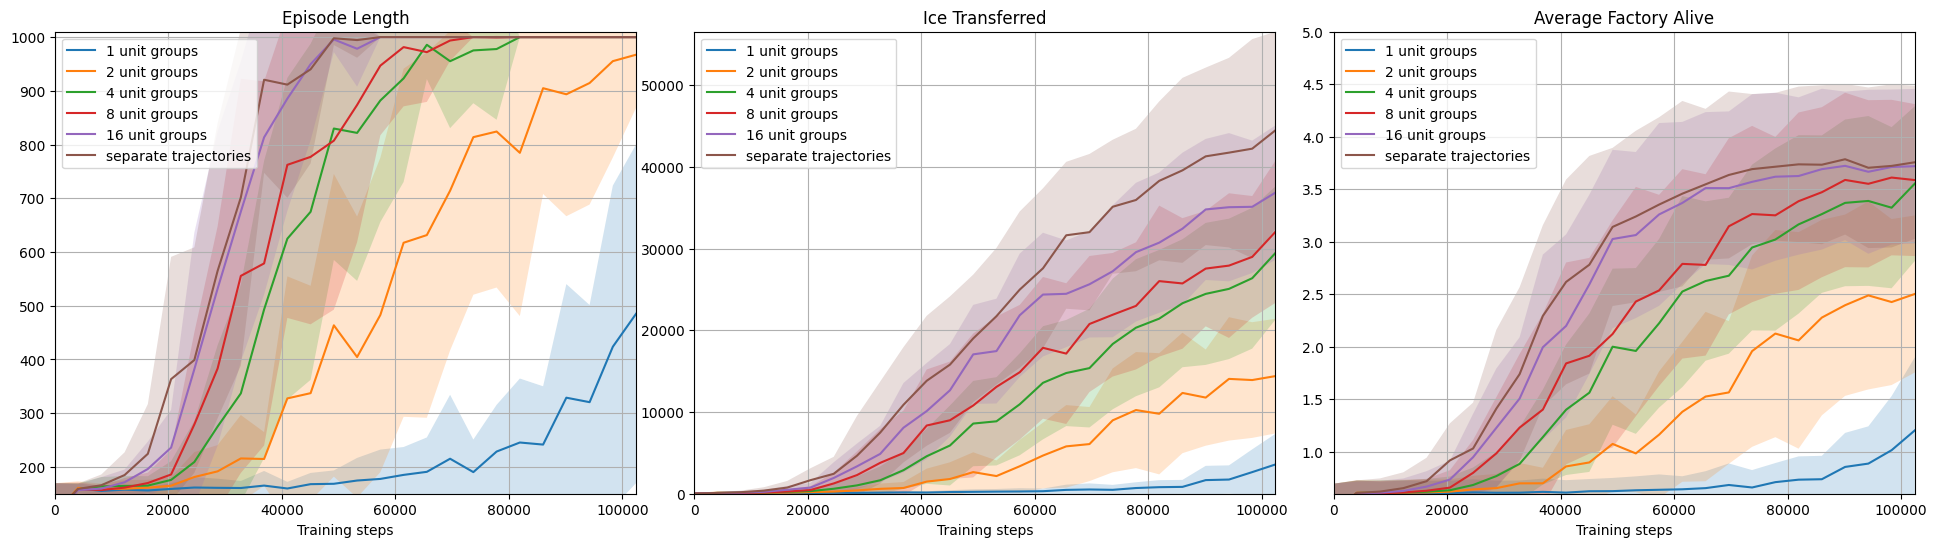
\includegraphics[width=0.95\linewidth]{images/results_hybrid/group_size/combined.png}
    \captionsetup{justification=justified, singlelinecheck=false, width=1\linewidth, labelfont=bf} 
    \caption[]{Plot comparing the performance of separating the global trajectory into $N$ separate trajectories in terms of the length of the episodes, ice transferred by units, and number of active factories. In addition to the test variants, the global and completely separate trajectory variants are also present. The figure indicates a positive correlation between the number of separate trajectories and the performance achieved on all metrics.}
    \label{fig:hybrid_results/group_size/combined}
\end{figure}

\begin{table}[ht]
    \footnotesize
    \renewcommand{\arraystretch}{1.2}%
    \begin{tabularx}{\textwidth}{|X|C{2.3cm}|C{2.3cm}|C{2.0cm}|C{2.0cm}|}
        \hline
\multicolumn{1}{|Y|}{\textbf{Group Name}} & \textbf{Final Ice Transferred} & \textbf{Final Episode Length} & \textbf{10\% of Episodes Finished by} & \textbf{95\% of Episodes Finished by} \\
        \hline
1 unit groups & 3,573 (3,753) & 485 (315) & 98,304 steps & - \\
2 unit groups & 14,388 (7,019) & 967 (99) & 57,344 steps & - \\
4 unit groups & 29,459 (8,150) & \textbf{1,000 (0)} & 36,864 steps & 77,824 steps \\
8 unit groups & 32,049 (8,701) & \textbf{1,000 (0)} & 32,768 steps & 61,440 steps \\
16 unit groups & 36,847 (8,224) & \textbf{1,000 (0)} & \textbf{28,672 steps} & 57,344 steps \\
separate trajectories & \textbf{44,472 (12,065)} & \textbf{1,000 (0)} & \textbf{28,672 steps} & \textbf{49,152 steps} \\
        \hline
    \end{tabularx}
    \medskip
    \captionsetup{justification=justified, singlelinecheck=false, width=1\linewidth, labelfont=bf} 
    \caption{Table comparing the performance of separating the global trajectory into $N$ separate trajectories. The metrics featured include the amount of ice transferred by units and the length of the episodes in the evaluation phase following the last training cycle. The table also contains the observed environment steps needed until the model reaches the maximum episode length in the specified percentage of evaluation environments. In addition to the test variants, the global and completely separate trajectory variants are also present. The table shows a massive jump in the final average episode length even by separating the global trajectory into two random groups. While the episode length metric reaches its maximum value with 4 unit groups, an increased convergence rate can be observed by using even more separate trajectories.}
    \label{tab:hybrid_results/group_size/combined}
\end{table}


\subsection{Trajectory Number Reduction}
\label{subsec:trajec_reduc}

\noindent The technique of \textbdd{trajectory separation} (\autoref{sec:trajectory-separation}) provides an optimized approach that enables efficient training of a centralized model for a multi-agent problem. However, it should be noted that the large number of trajectories does have certain limitations. Because the separated \textbdd{training examples} are tied to their respective environment steps, which are used to partition our \textbdd{mini-batches} during training, and considering that the number of trajectories can vary at each step, it is possible for the mini-batches to have an \textbdd{imbalanced number of training examples}. Given that the sizes of the matrices remain constant and padding values are used for inactive groups, this does not pose any issues regarding vectorization or memory utilization. Nevertheless, this phenomenon could potentially lead to an \textbdd{asymmetry} in the impact that each training example has on the policy loss, as the final loss is obtained by averaging all training examples. Steps with a large number of currently active groups will carry \textbdd{more significance}, whereas the impact of a group's example within a step with a low number of active groups will be \textbdd{more pronounced} compared to a group's example within a step with a higher population. This is because, on average, the former will be included in a mini-batch with fewer examples. Even if the mini-batch sizes were balanced, it would remain uncertain whether the \textbdd{increased number of trajectories} is \textbdd{advantageous} for the training process. The generation of a large number of training instances from the available environment steps introduces a \textbdd{regularization effect} to the model's training process, thereby reducing the influence of each individual instance. If the primary challenge associated with a single global trajectory is the complex action space and the \textbdd{incomprehensible singular reward value}, it is possible that by eliminating these factors, a reduced quantity of training examples may be sufficient to obtain convergence. Reducing the size of the batches while maintaining the same performance would further optimize our technique. In order to assess the impact of the aforementioned issues, we will employ two methodologies: \textbdd{agent grouping} (\autoref{sec:res-grouping}), wherein we will evaluate the performance attainable through various grouping criteria, and \textbdd{trajectory sample reduction} (\autoref{subsec:tsr}), wherein we will selectively utilize data from the top or bottom $N$ groups based on a specified metric for each step in the environment.

\subsubsection{Grouping}
\label{sec:res-grouping}

\noindent The results of the modulus test in \autoref{subsec:modulus-grouping} show a strong link between performance and the \textbdd{number of allowed separate trajectories}. The variant that was \textbdd{unconstrained} by any kind of grouping outperformed all the other variants. However, it raises the question of whether comparable performance can be attained with a \textbdd{bounded variant} by implementing a grouping rule that is beneficial for the training process. As shown in \autoref{fig:hybrid_results/group_rule/combined} and \autoref{tab:hybrid_results/group_rule/combined}, our experiment involved evaluating the effectiveness of three different grouping strategies: grouping by \textbdd{map segments} (\textttdb{"map quadrants"}), grouping by \textbdd{closest factories} (\textttdb{"closest factory"}), and grouping by \textbdd{closest heavy units} (\textttdb{"closest heavy"}). All of these groupings led to a \textbdd{bounded number of trajectories}, as the size of the map remains constant, and the number of factories can only vary between three and five. At first glance, the number of heavy units may appear to be limitless; however, the resources available to a factory only permit the production of a single heavy unit per factory. None of the groups that were tested were able to achieve performance comparable to that of the completely separated variant. Additionally, the \textbdd{number of groups remained a significant indicator of performance}. We used the \textbdd{randomly grouped} variants from \autoref{fig:hybrid_results/group_size/combined} (\textttdb{"4 unit groups"}, \textttdb{"8 unit groups"}) to see if non-random grouping rules can perform better than a random group assignment with the same number of separated trajectories. Unfortunately, all of the variants that were subjected to testing demonstrated lower performance or demonstrated comparable results to those assigned randomly. The sole exception was the \textttdb{"closest heavy"} variant; however, it still failed to outperform random assignment in terms of converging to the maximum episode length. The findings indicate that the approach of \textbdd{grouping} the trajectories of entities together in order to reduce the number of training examples \textbdd{yields poor performance}.

\begin{figure}[htbp]
    \centering
    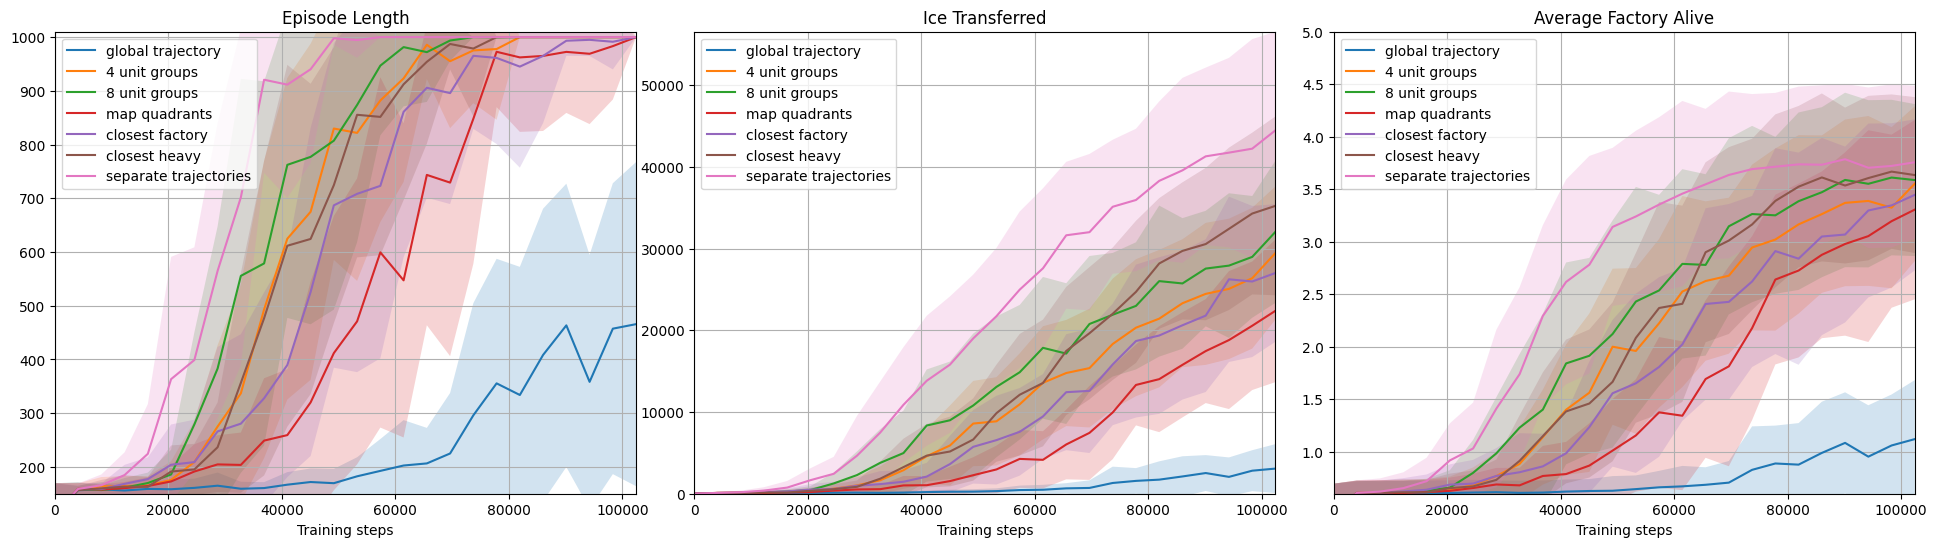
\includegraphics[width=0.95\linewidth]{images/results_hybrid/group_rule/combined.png}
    \captionsetup{justification=justified, singlelinecheck=false, width=1\linewidth, labelfont=bf} 
    \caption[]{Plot comparing the usage of different grouping rules in terms of the length of the episodes, ice transferred by units, and number of active factories. In addition to the test variants, the global and completely separate trajectory variants are also present. None of the tried variants managed to beat the separate trajectory variant in performance.}
    \label{fig:hybrid_results/group_rule/combined}
\end{figure}

\begin{table}[ht]
    \footnotesize
    \renewcommand{\arraystretch}{1.2}%
    \begin{tabularx}{\textwidth}{|X|C{2.3cm}|C{2.3cm}|C{2.0cm}|C{2.0cm}|}
        \hline
\multicolumn{1}{|Y|}{\textbf{Group Name}} & \textbf{Final Ice Transferred} & \textbf{Final Episode Length} & \textbf{10\% of Episodes Finished by} & \textbf{95\% of Episodes Finished by} \\
        \hline
global trajectory & 3,066 (2,996) & 466 (302) & 102,400 steps & - \\
4 unit groups & 29,459 (8,150) & \textbf{1,000 (0)} & 36,864 steps & 77,824 steps \\
8 unit groups & 32,049 (8,701) & \textbf{1,000 (0)} & 32,768 steps & 61,440 steps \\
map quadrants & 22,385 (8,733) & \textbf{1,000 (0)} & 53,248 steps & 98,304 steps \\
closest factory & 27,009 (8,420) & \textbf{1,000 (0)} & 45,056 steps & 94,208 steps \\
closest heavy & 35,224 (10,946) & \textbf{1,000 (0)} & 36,864 steps & 73,728 steps \\
separate trajectories & \textbf{44,472 (12,065)} & \textbf{1,000 (0)} & \textbf{28,672 steps} & \textbf{49,152 steps} \\
        \hline
    \end{tabularx}
    \medskip
    \captionsetup{justification=justified, singlelinecheck=false, width=1\linewidth, labelfont=bf} 
    \caption{Table comparing the usage of different grouping rules. The metrics featured include the amount of ice transferred by units and the length of the episodes in the evaluation phase following the last training cycle. The table also contains the observed environment steps needed until the model reaches the maximum episode length in the specified percentage of evaluation environments. In addition to the test variants, the global and completely separate trajectory variants are also present. While each grouping configuration performed better than the global trajectory variant, none could compete with the convergence rate of the completely separate trajectory variant. Grouping units by specific rules did not perform better than random grouping.}
    \label{tab:hybrid_results/group_rule/combined}
\end{table}

\subsubsection{Train Sample Reduction}
\label{subsec:tsr}

\noindent Given that all grouping methods performed less effectively than completely separate trajectories for all entities, we attempted an alternative approach to ensure a more consistent number of training examples at each step. Our technique, referred to as \textbdd{train sample reduction}, involves selecting the top $N$ examples from each step and training the model exclusively on those chosen examples. This action accomplishes two objectives. Firstly, it establishes an \textbdd{upper limit for the train examples}, thereby ensuring that the influence of each group's action remains relatively consistent, regardless of the number of other active groups. Secondly, in theory, by selecting only the most relevant examples at each step, we should be capable of \textbdd{accelerating the training process} of the model in terms of the number of environment steps and the amount of time required. In the following experiments, we utilize completely separated trajectories for all variants and perform the sample reduction solely on the train examples of units.

\bigskip

\noindent In order to first determine the optimal metric for selecting the desired subset of examples by, we conducted an experiment. We tried selecting the top $N=1$ samples by using various sampling techniques, including \textbdd{random sampling} (\textttdb{"random 1"}), \textbdd{top advantage value} (\textttdb{"top 1 advantage"}), \textbdd{top absolute advantage value} (\textttdb{"top 1 absolute advantage"}) and \textbdd{top return value} (\textttdb{"top 1 return"}). Among all of these variations, the subset that includes the examples with the \textbdd{greatest advantage value} achieved the highest performance, as evidenced by the results presented in \autoref{fig:hybrid_results/trajectory_sample_reduction/combined} and \autoref{tab:hybrid_results/trajectory_sample_reduction/combined}. Interestingly, utilizing solely the example with the \textbdd{most prominent advantage value} exhibited \textbdd{almost the same performance} as employing all of the train examples. Consequently, we decided to investigate sampling by this metric further, with different $N$ values.

\begin{figure}[htbp]
    \centering
    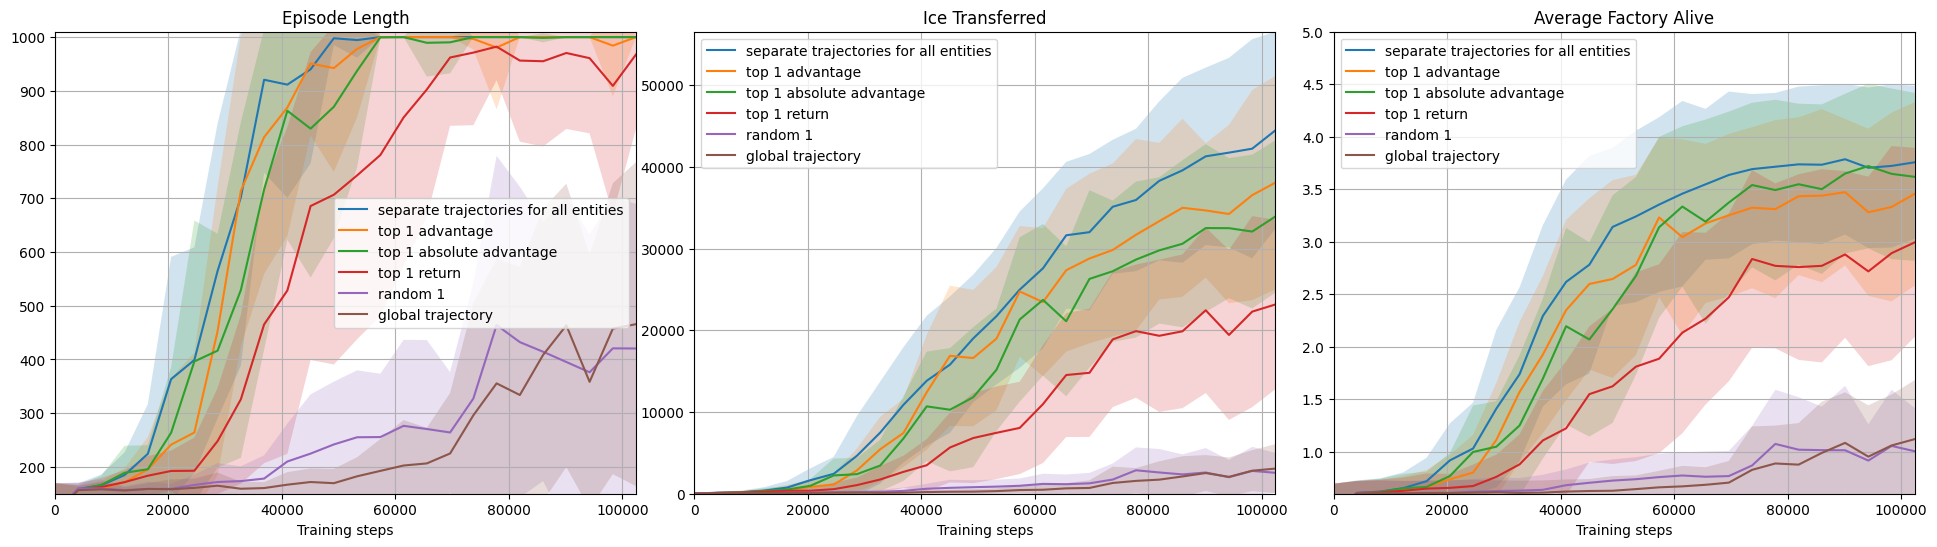
\includegraphics[width=0.95\linewidth]{images/results_hybrid/trajectory_sample_reduction/combined.png}
    \captionsetup{justification=justified, singlelinecheck=false, width=1\linewidth, labelfont=bf} 
    \caption[]{Plot comparing the different methods of trajectory sample reduction in terms of the length of the episodes, ice transferred by units, and number of active factories. In addition to the test variants, the global and completely separate trajectory variants are also present. Randomly selecting a single example at each step has the same effect as using a global trajectory. Out of all the sampling methods tried, selecting by advantage is the most prominent, leading to almost the same performance as using all data.}
    \label{fig:hybrid_results/trajectory_sample_reduction/combined}
\end{figure}

\begin{table}[ht]
    \footnotesize
    \renewcommand{\arraystretch}{1.2}%
    \begin{tabularx}{\textwidth}{|X|C{2.3cm}|C{2.3cm}|C{2.0cm}|C{2.0cm}|}
        \hline
\multicolumn{1}{|Y|}{\textbf{Group Name}} & \textbf{Final Ice Transferred} & \textbf{Final Episode Length} & \textbf{10\% of Episodes Finished by} & \textbf{95\% of Episodes Finished by} \\
        \hline
separate trajectories for all entities & \textbf{44,472 (12,065)} & \textbf{1,000 (0)} & \textbf{28,672 steps} & \textbf{49,152 steps} \\
top 1 advantage & 38,072 (13,071) & \textbf{1,000 (0)} & 32,768 steps & 57,344 steps \\
top 1 absolute advantage & 33,926 (9,324) & \textbf{1,000 (0)} & 32,768 steps & 57,344 steps \\
top 1 return & 23,156 (10,369) & 968 (138) & 40,960 steps & - \\
random 1 & 2,550 (2,434) & 420 (269) & 77,824 steps & - \\
global trajectory & 3,066 (2,996) & 466 (302) & 102,400 steps & - \\
        \hline
    \end{tabularx}
    \medskip
    \captionsetup{justification=justified, singlelinecheck=false, width=1\linewidth, labelfont=bf} 
    \caption{Table comparing the different methods of trajectory sample reduction. The metrics featured include the amount of ice transferred by units and the length of the episodes in the evaluation phase following the last training cycle. The table also contains the observed environment steps needed until the model reaches the maximum episode length in the specified percentage of evaluation environments. In addition to the test variants, the global and completely separate trajectory variants are also present. The table shows how selecting a single train example from each step by the right metric could approximate the training performance on all data. The advantage value proved to be the best metric for sampling.}
    \label{tab:hybrid_results/trajectory_sample_reduction/combined}
\end{table}

\bigskip

\noindent We tested the impact of selecting different numbers of examples with the highest advantage values from each environment step. Specifically, we tested the effects of taking 1, 2, 4, 8, and 16 such examples. The results are presented in \autoref{fig:hybrid_results/trajectory_sample_reduction_advantage/combined} and \autoref{tab:hybrid_results/trajectory_sample_reduction_advantage/combined}. Curiously, the inclusion of additional examples does not appear to significantly enhance performance. In fact, the rate of convergence is \textbdd{slightly hindered} when the sample size is increased from 4 to 16. This implies that the \textbdd{significance of an entity's action} may be \textbdd{diminished} by the multitude of other actions currently occurring in the surrounding environment, making the action less dominant in the loss calculation. By reducing the number of separate training examples and subsequently removing unnecessary data beforehand, we can help the convergence of the model. The slight edge exhibited by the sampled variants could also potentially be attributed to avoiding the problem of changing batch sizes, although a definitive conclusion cannot be drawn. We also cannot exclude the possibility that the observed, relatively small differences are due to \textbdd{sampling noise}.

\begin{figure}[ht]
    \centering
    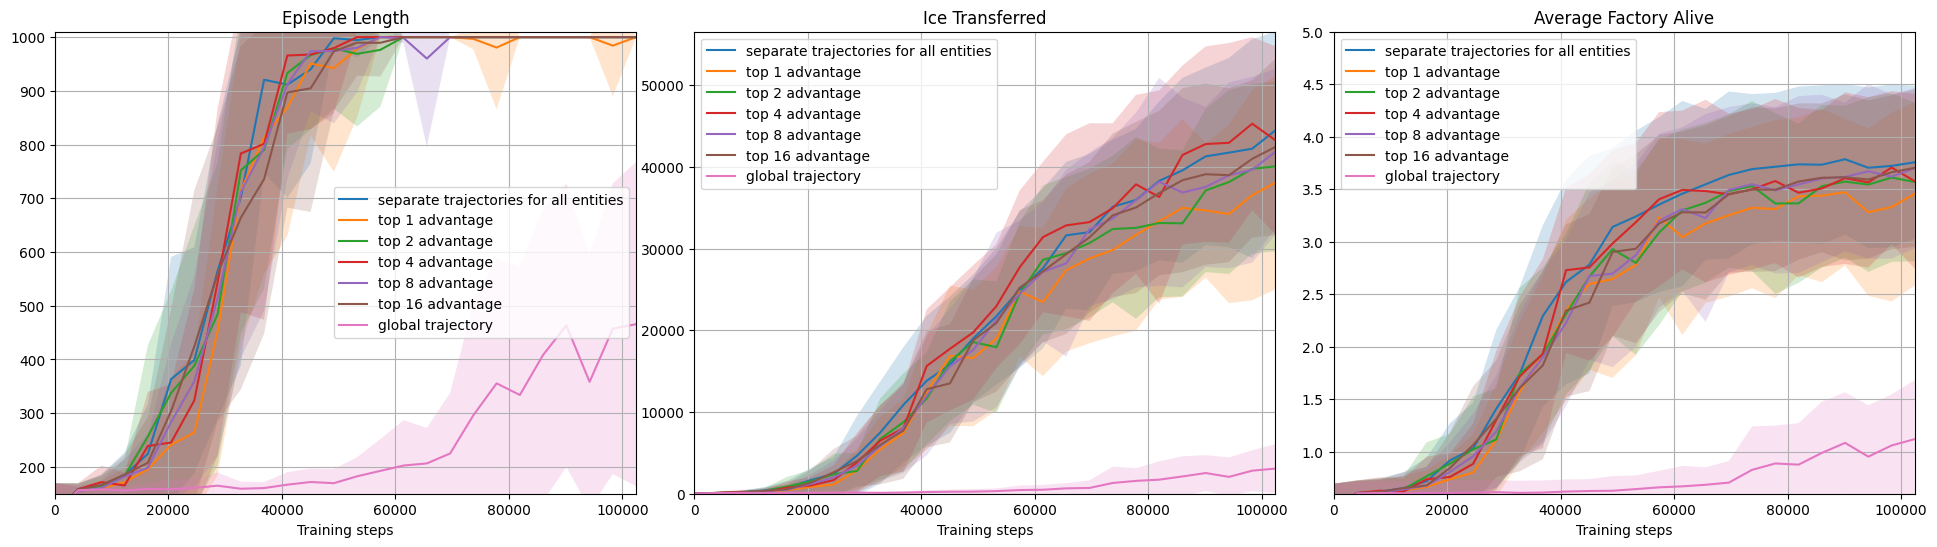
\includegraphics[width=0.95\linewidth]{images/results_hybrid/trajectory_sample_reduction_advantage/combined.png}
    \captionsetup{justification=justified, singlelinecheck=false, width=1\linewidth, labelfont=bf} 
    \caption[]{Plot comparing the performance of sampling train examples based on the advantage values in terms of the length of the episodes, ice transferred by units, and number of active factories. In addition to the test variants, the global and completely separate trajectory variants are also present. Increasing the number of sampled values appears to have minimal effect on performance, leading us to believe that the main benefit of utilizing a larger training set is to find outstandingly beneficial examples.}
    \label{fig:hybrid_results/trajectory_sample_reduction_advantage/combined}
\end{figure}

\begin{table}[ht]
    \footnotesize
    \renewcommand{\arraystretch}{1.2}%
    \begin{tabularx}{\textwidth}{|X|C{2.3cm}|C{2.3cm}|C{2.0cm}|C{2.0cm}|}
        \hline
\multicolumn{1}{|Y|}{\textbf{Group Name}} & \textbf{Final Ice Transferred} & \textbf{Final Episode Length} & \textbf{10\% of Episodes Finished by} & \textbf{95\% of Episodes Finished by} \\
        \hline
separate trajectories for all entities & \textbf{44,472 (12,065)} & \textbf{1,000 (0)} & 28,672 steps & \textbf{49,152 steps} \\
top 1 advantage & 38,072 (13,071) & \textbf{1,000 (0)} & 32,768 steps & 57,344 steps \\
top 2 advantage & 40,053 (10,402) & \textbf{1,000 (0)} & \textbf{24,576 steps} & 61,440 steps \\
top 4 advantage & 43,246 (11,518) & \textbf{1,000 (0)} & 28,672 steps & \textbf{49,152 steps} \\
top 8 advantage & 41,855 (10,159) & \textbf{1,000 (0)} & 28,672 steps & 57,344 steps \\
top 16 advantage & 42,433 (10,792) & \textbf{1,000 (0)} & \textbf{24,576 steps} & 53,248 steps \\
global trajectory & 3,066 (2,996) & 466 (302) & 102,400 steps & - \\
        \hline
    \end{tabularx}
    \medskip
    \captionsetup{justification=justified, singlelinecheck=false, width=1\linewidth, labelfont=bf} 
    \caption{Table comparing the performance of sampling train examples based on the advantage values. The metrics featured include the amount of ice transferred by units and the length of the episodes in the evaluation phase following the last training cycle. The table also contains the observed environment steps needed until the model reaches the maximum episode length in the specified percentage of evaluation environments. In addition to the test variants, the global and completely separate trajectory variants are also present. Increasing the number of advantage-sampled values did not appear to have a significant effect on performance.}
    \label{tab:hybrid_results/trajectory_sample_reduction_advantage/combined}
\end{table}

\bigskip

\noindent We were also interested in investigating the performance that can be achieved through \textbdd{random sampling}. We conducted an experiment examining the performance of different numbers of random samples, specifically 1, 2, 4, 8, and 16. The aforementioned variants were subsequently compared to the established, completely separate, and global variants. The results are available in \autoref{fig:hybrid_results/trajectory_sample_reduction_random/combined} and \autoref{tab:hybrid_results/trajectory_sample_reduction_random/combined}. Using a random sampling approach cannot provide comparable performance to utilizing the entire dataset. As expected, the performance improved as we increased the number of sampled examples, consistent with the random grouping observed in the trajectory separation experiment (\autoref{subsec:modulus-grouping}).

\begin{figure}[htbp]
    \centering
    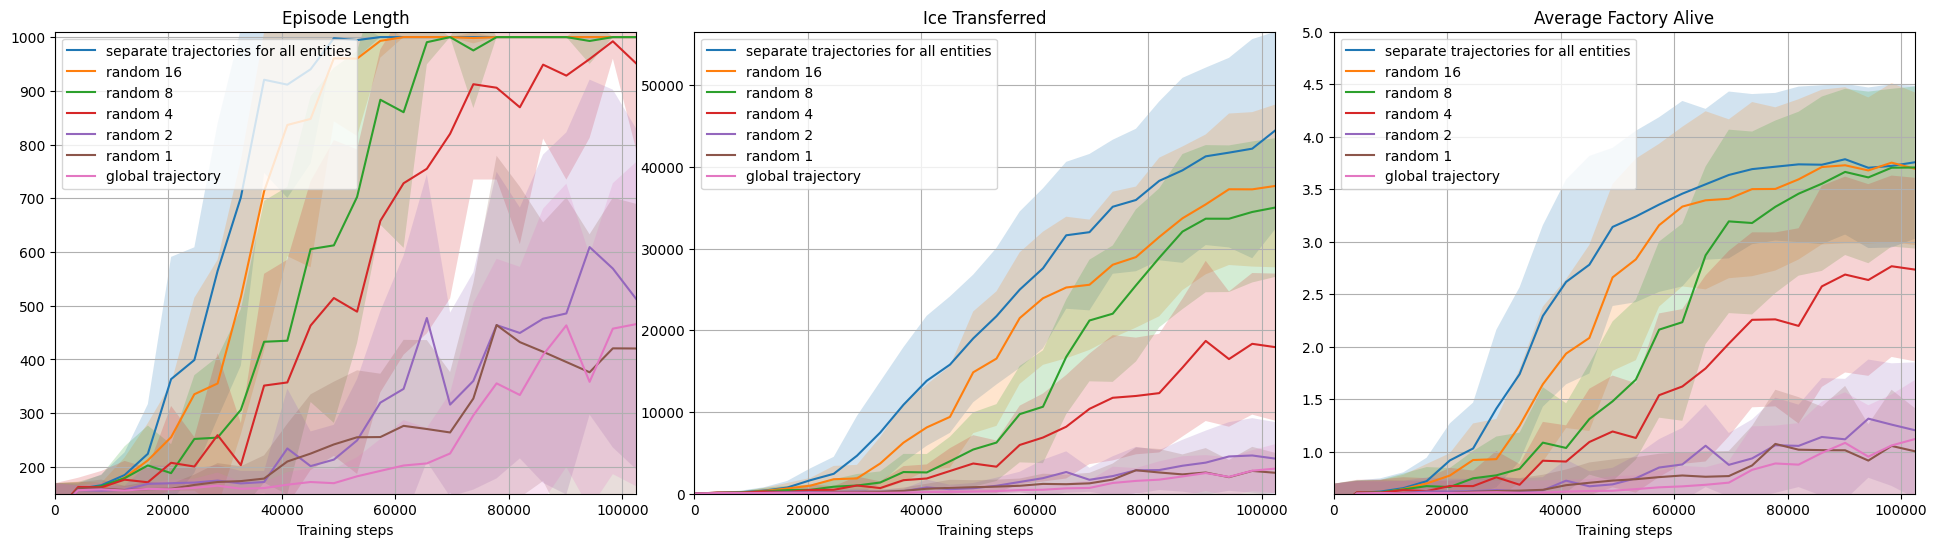
\includegraphics[width= 0.95\linewidth]{images/results_hybrid/trajectory_sample_reduction_random/combined.png}
    \captionsetup{justification=justified, singlelinecheck=false, width=1\linewidth, labelfont=bf} 
    \caption[]{Plot showcasing the performance of random train example sampling in terms of the length of the episodes, ice transferred by units, and number of active factories. In addition to the test variants, the global and completely separate trajectory variants are also present. As expected, more randomly sampled trajectories caused better performance.}
    \label{fig:hybrid_results/trajectory_sample_reduction_random/combined}
\end{figure}

\begin{table}[ht]
    \footnotesize
    \renewcommand{\arraystretch}{1.2}%
    \begin{tabularx}{\textwidth}{|X|C{2.3cm}|C{2.3cm}|C{2.0cm}|C{2.0cm}|}
        \hline
\multicolumn{1}{|Y|}{\textbf{Group Name}} & \textbf{Final Ice Transferred} & \textbf{Final Episode Length} & \textbf{10\% of Episodes Finished by} & \textbf{95\% of Episodes Finished by} \\
        \hline
separate trajectories for all entities & \textbf{44,472 (12,065)} & \textbf{1,000 (0)} & \textbf{28,672 steps} & \textbf{49,152 steps} \\
random 16 & 37,665 (9,965) & \textbf{1,000 (0)} & 32,768 steps & 61,440 steps \\
random 8 & 35,022 (8,492) & \textbf{1,000 (0)} & 45,056 steps & 69,632 steps \\
random 4 & 17,927 (9,007) & 951 (160) & 45,056 steps & - \\
random 2 & 4,284 (4,475) & 513 (317) & 77,824 steps & - \\
random 1 & 2,550 (2,434) & 420 (269) & 77,824 steps & - \\
global trajectory & 3,066 (2,996) & 466 (302) & 102,400 steps & - \\
        \hline
    \end{tabularx}
    \medskip
    \captionsetup{justification=justified, singlelinecheck=false, width=1\linewidth, labelfont=bf} 
    \caption{Table showcasing the performance of random train example sampling. The metrics featured include the amount of ice transferred by units and the length of the episodes in the evaluation phase following the last training cycle. The table also contains the observed environment steps needed until the model reaches the maximum episode length in the specified percentage of evaluation environments. In addition to the test variants, the global and completely separate trajectory variants are also present. As expected, more sampled trajectories resulted in better performance.}
    \label{tab:hybrid_results/trajectory_sample_reduction_random/combined}
\end{table}

\subsubsection{Emphasizing Data Quality over Quantity}
\noindent In \autoref{subsec:tsr}, we observed that the act of sampling a \textbdd{single training example} from an environment step with separate trajectories \textbdd{yields the same suboptimal outcome} as utilizing a \textbdd{global trajectory}. Moreover, employing a sample selection method based on a reward-like metric can \textbdd{yield comparable performance} to training on the \textbdd{entire dataset}. From our perspective, this suggests the significance of \textbdd{data quality} over \textbdd{data quantity}. In order to further examine this concept, we conducted a comparison between \textbdd{train sample reduction} and \textbdd{random grouping} (\autoref{subsec:modulus-grouping}). The results are presented in \autoref{fig:hybrid_results/grouping_vs_tsr/combined} and \autoref{tab:hybrid_results/grouping_vs_tsr/combined}. In this study, the two observed methods of training sample reduction were \textbdd{random sampling} (\textttdb{"random 1 samples"}, \textttdb{"random 4 samples"}), since it is the most easily comparable to \textbdd{random grouping} (\textttdb{"1 unit groups"}, \textttdb{"4 unit groups"}), and \textbdd{advantage-based selection} (\textttdb{"top 1 advantage"}, \textttdb{"top 4 advantage"}), which achieved the best performance in the trajectory separation test (\autoref{subsec:tsr}). We can derive from these charts that \textbdd{increasing the number of training examples} does \textbdd{not necessarily} lead to \textbdd{improved performance}, as advantage-based selection managed to beat random sampling even with a smaller sample size. This shows that the primary purpose of using a large amount of data in reinforcement learning is to \textbdd{identify actions} that are clearly \textbdd{more favorable}. In the experiment, both grouping and trajectory separation resulted in a maximum of 4 training examples per environment step. However, it is important to note that grouping incorporates data from all entities, although it poses challenges in terms of learnability, as discussed in \autoref{subsec:methodcomp}. This \textbdd{increased complexity of the training data} leads to a \textbdd{significant decrease in performance}, to the extent that even random sampling, which only includes a small subset of all entity data, can achieve similar performance. Furthermore, when we switch to advantage-based sampling, which learns only from the pre-selected most relevant examples, its training massively outperforms the grouped variant's. This further confirms the significance of data quality.

\begin{figure}[htbp]
    \centering
    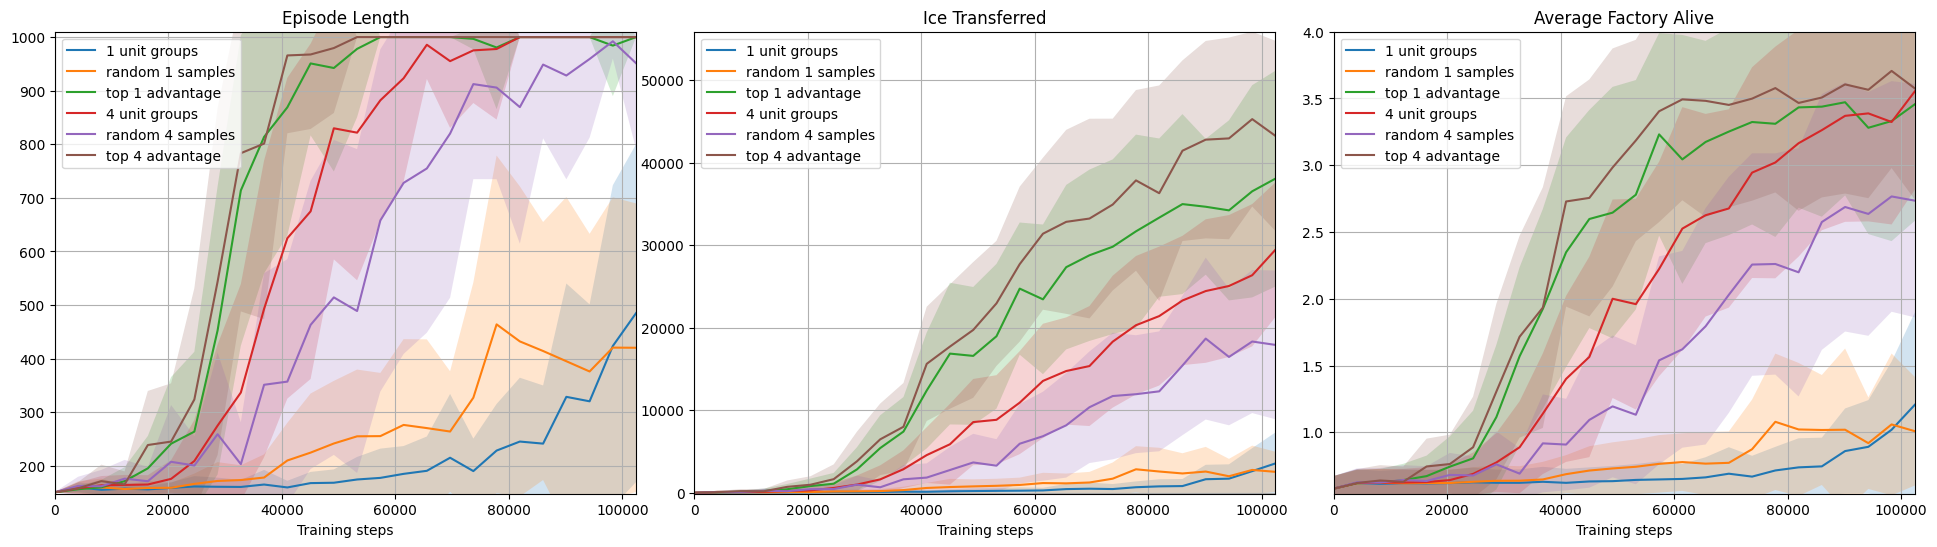
\includegraphics[width=0.95\linewidth]{images/results_hybrid/grouping_vs_tsr/combined.png}
    \captionsetup{justification=justified, singlelinecheck=false, width=1\linewidth, labelfont=bf} 
    \caption[]{Plot comparing random grouping, random sampling, and advantage-based sampling in terms of the length of the episodes, ice transferred by units, and number of active factories. Sampling by advantage outperforms both random grouping and random sampling, even if the advantage-based sampling contains fewer trajectories, suggesting greater importance of data quality than quantity.}
    \label{fig:hybrid_results/grouping_vs_tsr/combined}
\end{figure}

\begin{table}[ht]
    \footnotesize
    \renewcommand{\arraystretch}{1.2}%
    \begin{tabularx}{\textwidth}{|X|C{2.3cm}|C{2.3cm}|C{2.0cm}|C{2.0cm}|}
        \hline
\multicolumn{1}{|Y|}{\textbf{Group Name}} & \textbf{Final Ice Transferred} & \textbf{Final Episode Length} & \textbf{10\% of Episodes Finished by} & \textbf{95\% of Episodes Finished by} \\
        \hline
1 unit groups & 3,573 (3,753) & 485 (315) & 98,304 steps & - \\
random 1 samples & 2,550 (2,434) & 420 (269) & 77,824 steps & - \\
top 1 advantage & 38,072 (13,071) & \textbf{1,000 (0)} & 32,768 steps & 57,344 steps \\
4 unit groups & 29,459 (8,150) & \textbf{1,000 (0)} & 36,864 steps & 77,824 steps \\
random 4 samples & 17,927 (9,007) & 951 (160) & 45,056 steps & - \\
top 4 advantage & \textbf{43,246 (11,518)} & \textbf{1,000 (0)} & \textbf{28,672 steps} & \textbf{49,152 steps} \\
        \hline
    \end{tabularx}
    \medskip
    \captionsetup{justification=justified, singlelinecheck=false, width=1\linewidth, labelfont=bf} 
    \caption{Table comparing random grouping, random sampling, and advantage-based sampling. The metrics featured include the amount of ice transferred by units and the length of the episodes in the evaluation phase following the last training cycle. The table also contains the observed environment steps needed until the model reaches the maximum episode length in the specified percentage of evaluation environments. The advantage-based sampling managed to outperform the other variants in all metrics, even with fewer training examples, while the random sampling underperformed random grouping.}
    \label{tab:hybrid_results/grouping_vs_tsr/combined}
\end{table}


\subsection{Method Components}
\label{subsec:methodcomp}

\noindent Although the results obtained in \autoref{sec:trajectory-separation} seem impressive, it is \textbdd{challenging to identify} the specific factor that has led to such a substantial \textbdd{improvement in performance}. Based on our current understanding, the act of separating the trajectories leads to four notable enhancements in the training process. The process generates additional \textbdd{training examples} from the same environmental steps, thereby enhancing the model's ability to acquire broader policies at an accelerated rate through increased exploration. Another, perhaps the most noteworthy advantage, is the eradication of the \textbdd{reinforcement of undesirable behavior}. Such reinforcement could arise if one entity performs an action that results in a high advantage value while another entity behaves in a manner that is suboptimal for the team's success but doesn't get punished by enough negative advantage. In this case, the incorrect action would be reinforced alongside the positive action. By employing separate trajectories with \textbdd{localized rewards}, the occurrence of such events can be prevented. Our method also \textbdd{avoids calculating} advantage from steps where the \textbdd{original performing entity is no longer active}. If only a single trajectory were utilized, there would be no way to keep track of the status and reward of individual entities. Within highly dynamic environments, such as Lux, this phenomenon leads to a somewhat \textbdd{misleading calculation} due to the significant probability that the units and factories currently in existence will not persist until the conclusion of the episode. Consequently, it is \textbdd{impossible to determine} whether their actions in the present have truly contributed to \textbdd{any real advantage}. By keeping the rewards separate, we ensure that the entity receives credit for its immediate and observable efforts, both in the present and future. Lastly, separate trajectories result in separate \textbdd{advantage} calculations and separate \textbdd{critic value} outputs for all groups. Estimating the \textbdd{entire game state} in order to provide a final \textbdd{global value} is a significantly \textbdd{more complex} task for the model compared to predicting multiple values based on \textbdd{local observations}. Within this subsection, we examine the \textbdd{different components} of trajectory separation to determine which part has the greatest impact on enhancing performance.

\subsubsection{Inividual Components}
\label{subsec:individual-components}

\noindent Our initial hypothesis was that the most crucial components that needed to be separated were the \textbdd{reward}, \textbdd{terminal state} indication, \textbdd{critic value}, \textbdd{log probabilities}, and \textbdd{entropy} values. Therefore, we conducted a series of experiments where we systematically removed the separation of these components one by one. The purpose of these experiments was to observe the impact of each component's loss on the model's overall performance.

\bigskip

\noindent Both the \textbdd{reward} and \textbdd{critic} values are essential for the computation of the \textbdd{advantage}, an integral component of the Proximal Policy Optimization (\autoref{sec:ppo}) algorithm. Therefore, we decided to start with removing separation between these values. The results can be seen in \autoref{fig:hybrid_results/components/combined_rew} and \autoref{tab:hybrid_results/components/combined_rew}. The metrics for the \textttdb{"separate trajectories, global reward"} variant indicate that the utilization of separate trajectories with global rewards leads to a notable decrease in convergence speed, in comparison to separate trajectories with \textbdd{localized rewards}. This negative effect was expected since the absence of separated rewards hinders the model's ability to \textbdd{identify the specific actions} undertaken by the units and factories that led to the rewards received. Consequently, this issue aligns with the problem outlined in \autoref{par:global-rew}. In order to achieve efficient global advantage calculation, the critic head of the model must learn how to \textbdd{predict the performance of the entire team} rather than solely relying on predictions based on the local observations of individual entities. The decline in performance due to losing the ability to calculate \textbdd{critic value} predictions based on local information is further indicated by the \textttdb{"separate trajectories, global critic"} variant. The agents were able to sustain the operation of the factories for up to 1,000 steps in most environments, albeit at a slower pace, demonstrating how \textbdd{harder} it is for the model to work \textbdd{solely from global information}. Only when we remove both the \textbdd{critic values} and \textbdd{rewards} in test \textttdb{"separate trajectories, global advantage"} do we observe a reduction in performance to the level of a single global trajectory. A fully global \textbdd{advantage} calculation results in the \textbdd{same advantage value output for all entities}, meaning there is no way to differentiate between positive and negative actions under the same step, massively slowing down the training. Following this modification, the only difference in the policy loss between the entities is the \textbdd{probability ratios}, which fail to provide us any information about the desired direction and magnitude of policy updates. Due to the abovementioned factors, we believe that separate rewards hold significant importance. The impact of their effect is further examined in \autoref{subsubsec:rewardass}.

\bigskip

\noindent The outcomes following the elimination of the remaining separation components, namely the termination flags and the action probabilities, are observable in \autoref{fig:hybrid_results/components/combined_misc} and \autoref{tab:hybrid_results/components/combined_misc}. The fact that the performance remained consistent even after the removal of the separated \textbdd{terminal state flags} was unexpected and surprising to us. This group can be seen under the name \textttdb{"separate trajectories, global dones"}. Given that the trajectories are separated, and \textbdd{only currently active entities receive rewards}, indicating episode terminations prematurely at the destruction of an entity is somewhat \textbdd{redundant} since there will be no future rewards assigned to them that could skew the return calculation anyway. The act of indicating the inactivity of a group of agents is more logical in situations where the group has the potential to become active once again, particularly in cases where multiple entities are present within the same group. If all entities within the group are destroyed, but subsequently, a new entity is assigned, it is possible for the group to regain its activity. Whether stopping the future reward calculation between these two group states is beneficial is yet to be explored. The separation of \textbdd{distribution entropy values} does not appear to have any significance, as these values are ultimately combined into a single value to calculate the entropy loss regularization term. What massively degraded performance, however, was the removal of the \textbdd{separated log probabilities}. Through the aggregation of log probabilities, the gradients can \textbdd{propagate across} the action calculations of \textbdd{all entities}. Similarly to the combined advantage value, this global gradient propagation causes weight adjustments based on the whole team's performance, making it impossible to separate individual contributions. This observation shows the necessity of utilizing separate action probabilities in order to achieve optimal training.

\begin{figure}[htbp]
    \centering
    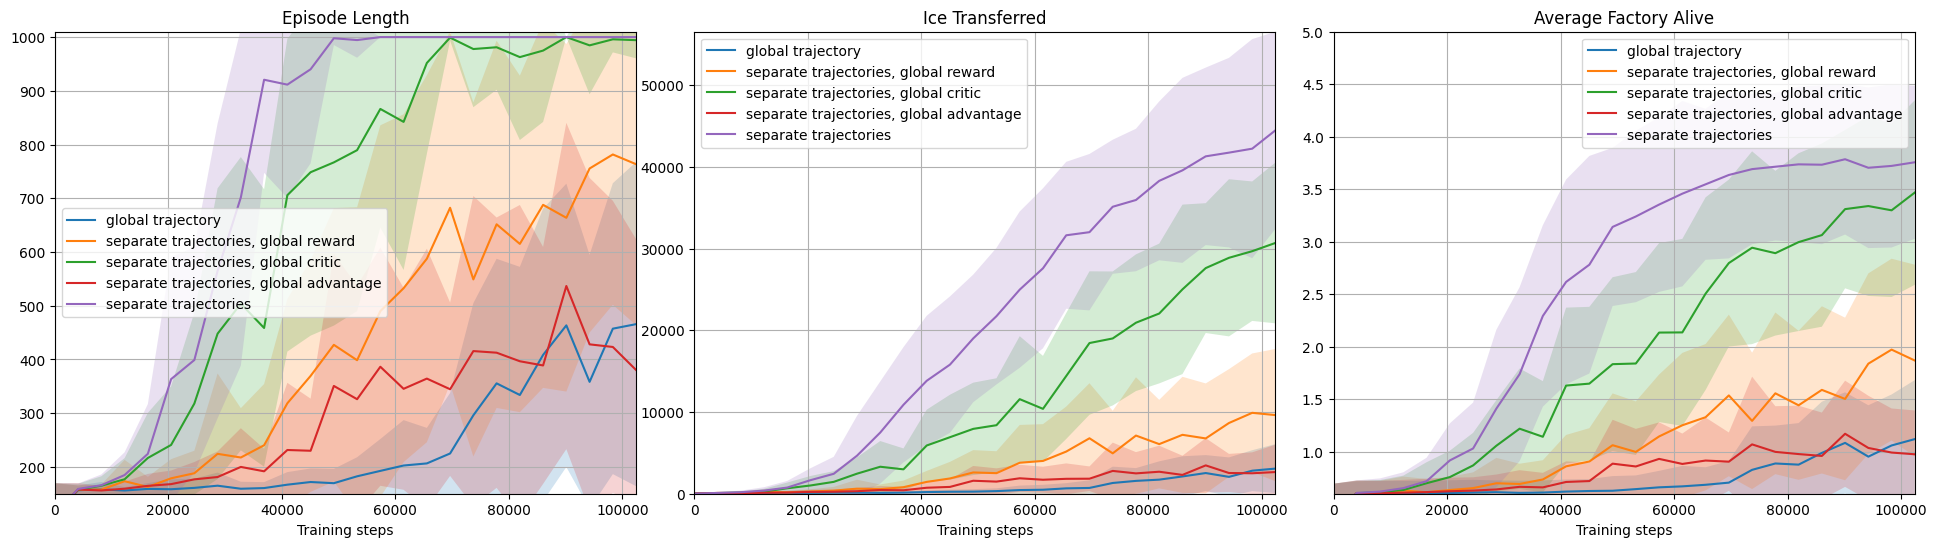
\includegraphics[width=0.95\linewidth]{images/results_hybrid/components/combined_rew.png}
    \captionsetup{justification=justified, singlelinecheck=false, width=1\linewidth, labelfont=bf} 
    \caption[]{Plot comparing the removal of separated components relevant to the advantage calculation in terms of the length of the episodes, ice transferred by units, and number of active factories. In addition to the test variants, the global and completely separate trajectory variants are also present. The separated reward plays a significant role but doesn't account for the whole performance boost. Removing separated critic value predictions and separated rewards together results in a similar performance to a single global trajectory.}
    \label{fig:hybrid_results/components/combined_rew}
\end{figure}

\begin{table}[ht]
    \footnotesize
    \renewcommand{\arraystretch}{1.2}%
    \begin{tabularx}{\textwidth}{|X|C{2.3cm}|C{2.3cm}|C{2.0cm}|C{2.0cm}|}
        \hline
\multicolumn{1}{|Y|}{\textbf{Group Name}} & \textbf{Final Ice Transferred} & \textbf{Final Episode Length} & \textbf{10\% of Episodes Finished by} & \textbf{95\% of Episodes Finished by} \\
        \hline
global trajectory & 3,066 (2,996) & 466 (302) & 102,400 steps & - \\
separate trajectories, global reward & 9,614 (8,094) & 763 (300) & 53,248 steps & - \\
separate trajectories, global critic & 30,687 (9,844) & 994 (34) & 40,960 steps & 69,632 steps \\
separate trajectories, global advantage & 2,643 (3,353) & 380 (244) & 73,728 steps & - \\
separate trajectories & \textbf{44,472 (12,065)} & \textbf{1,000 (0)} & \textbf{28,672 steps} & \textbf{49,152 steps} \\
        \hline
    \end{tabularx}
    \medskip
    \captionsetup{justification=justified, singlelinecheck=false, width=1\linewidth, labelfont=bf} 
    \caption{Table comparing the removal of separated components relevant to the advantage calculation. The metrics featured include the amount of ice transferred by units and the length of the episodes in the evaluation phase following the last training cycle. The table also contains the observed environment steps needed until the model reaches the maximum episode length in the specified percentage of evaluation environments. In addition to the test variants, the global and completely separate trajectory variants are also present. Removing the separation of rewards and critic values caused a significant performance decrease. Reward appears to be the most important component.}
    \label{tab:hybrid_results/components/combined_rew}
\end{table}

\begin{figure}[htbp]
    \centering
    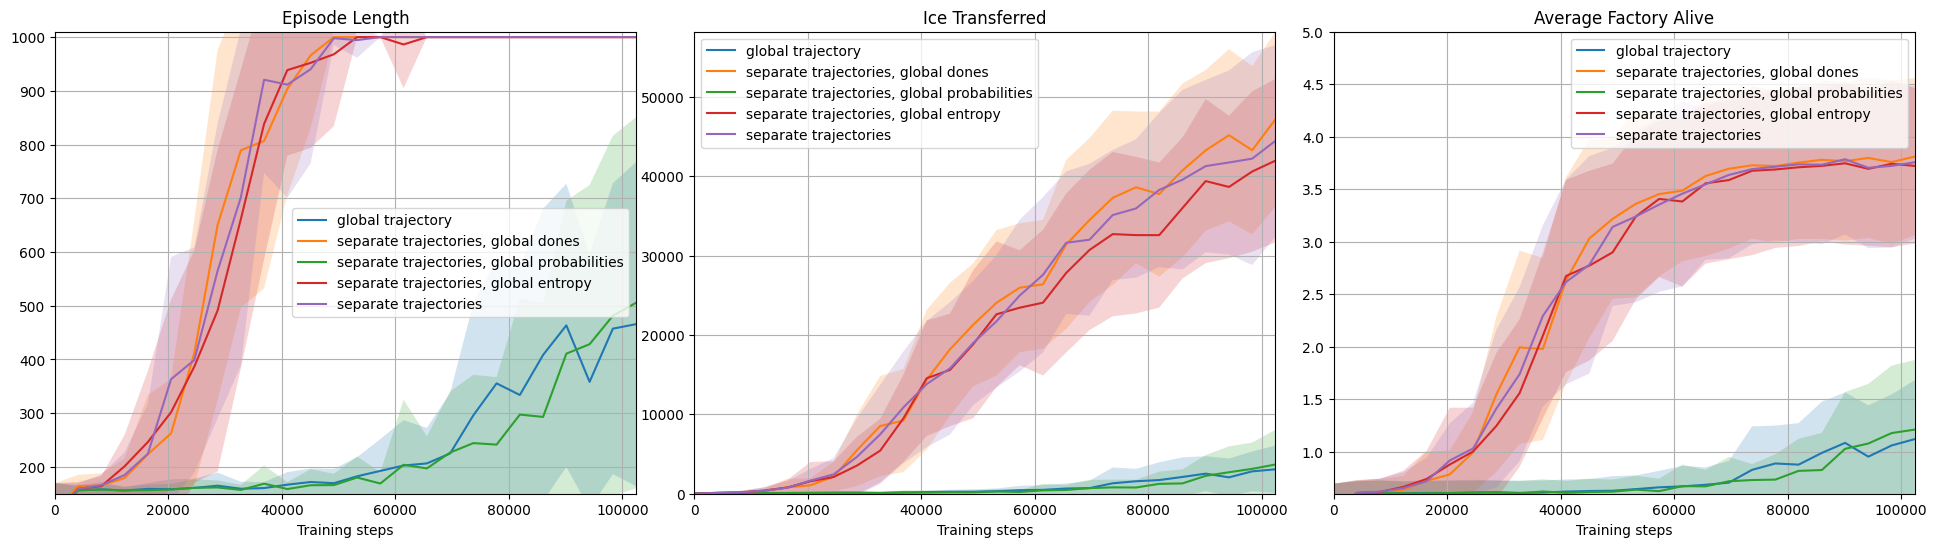
\includegraphics[width=0.95\linewidth]{images/results_hybrid/components/combined_misc.png}
    \captionsetup{justification=justified, singlelinecheck=false, width=1\linewidth, labelfont=bf} 
    \caption[]{Plot comparing the removal of other separated components in terms of the length of the episodes, ice transferred by units, and number of active factories. In addition to the test variants, the global and completely separate trajectory variants are also present. Aggregating the action probabilities globally degrades the model's performance to the level of a single global trajectory.}
    \label{fig:hybrid_results/components/combined_misc}
\end{figure}

\begin{table}[ht]
    \footnotesize
    \renewcommand{\arraystretch}{1.2}%
    \begin{tabularx}{\textwidth}{|X|C{2.3cm}|C{2.3cm}|C{2.0cm}|C{2.0cm}|}
        \hline
\multicolumn{1}{|Y|}{\textbf{Group Name}} & \textbf{Final Ice Transferred} & \textbf{Final Episode Length} & \textbf{10\% of Episodes Finished by} & \textbf{95\% of Episodes Finished by} \\
        \hline
global trajectory & 3,066 (2,996) & 466 (302) & 102,400 steps & - \\
separate trajectories, global dones & \textbf{47,201 (11,018)} & \textbf{1,000 (0)} & \textbf{28,672 steps} & \textbf{49,152 steps} \\
separate trajectories, global probabilities & 3,673 (4,372) & 506 (345) & 98,304 steps & - \\
separate trajectories, global entropy & 41,970 (10,305) & \textbf{1,000 (0)} & \textbf{28,672 steps} & 53,248 steps \\
separate trajectories & 44,472 (12,065) & \textbf{1,000 (0)} & \textbf{28,672 steps} & \textbf{49,152 steps} \\
        \hline
    \end{tabularx}
    \medskip
    \captionsetup{justification=justified, singlelinecheck=false, width=1\linewidth, labelfont=bf} 
    \caption{Table comparing the removal of other separated components. The metrics featured include the amount of ice transferred by units and the length of the episodes in the evaluation phase following the last training cycle. The table also contains the observed environment steps needed until the model reaches the maximum episode length in the specified percentage of evaluation environments. In addition to the test variants, the global and completely separate trajectory variants are also present. The table demonstrates the importance of separate action probabilities in order to limit the gradient flow to only relevant parts of the network during training.}
    \label{tab:hybrid_results/components/combined_misc}
\end{table}

\subsubsection{Reward Assignment}
\label{subsubsec:rewardass}

\noindent Based on the findings reported in \autoref{subsec:individual-components}, which indicated a significant impact of reward separation on performance, our objective was to investigate the importance of \textbdd{localized rewards}. To achieve this, we conducted an experiment combining the local, separated reward with the aggregated \textbdd{global reward}. Agents were allocated different percentages of their own rewards, specifically 0\%, 50\%, 75\%, and 100\% of their own rewards, with the remaining percentages being made up by the global reward. As evident from the data presented in \autoref{fig:hybrid_results/reward_assignment/combined} and \autoref{tab:hybrid_results/reward_assignment/combined}, the variant with completely separate reward values demonstrates superior performance compared to the other variants. Utilizing 25\% of the global rewards appears to result in convergence to an episode length of 1,000 at approximately the same step. Nevertheless, it gets outperformed in the \textbdd{ice transferred} and \textbdd{average factory alive} metrics by the completely separate variant. The variant that receives 50\% global rewards achieves the maximum episode length on average, whereas the variant that solely relies on global rewards fails to converge even after 100,000 steps. This experiment provides additional evidence to support the significance of localized rewards.

\begin{figure}[htbp]
    \centering
    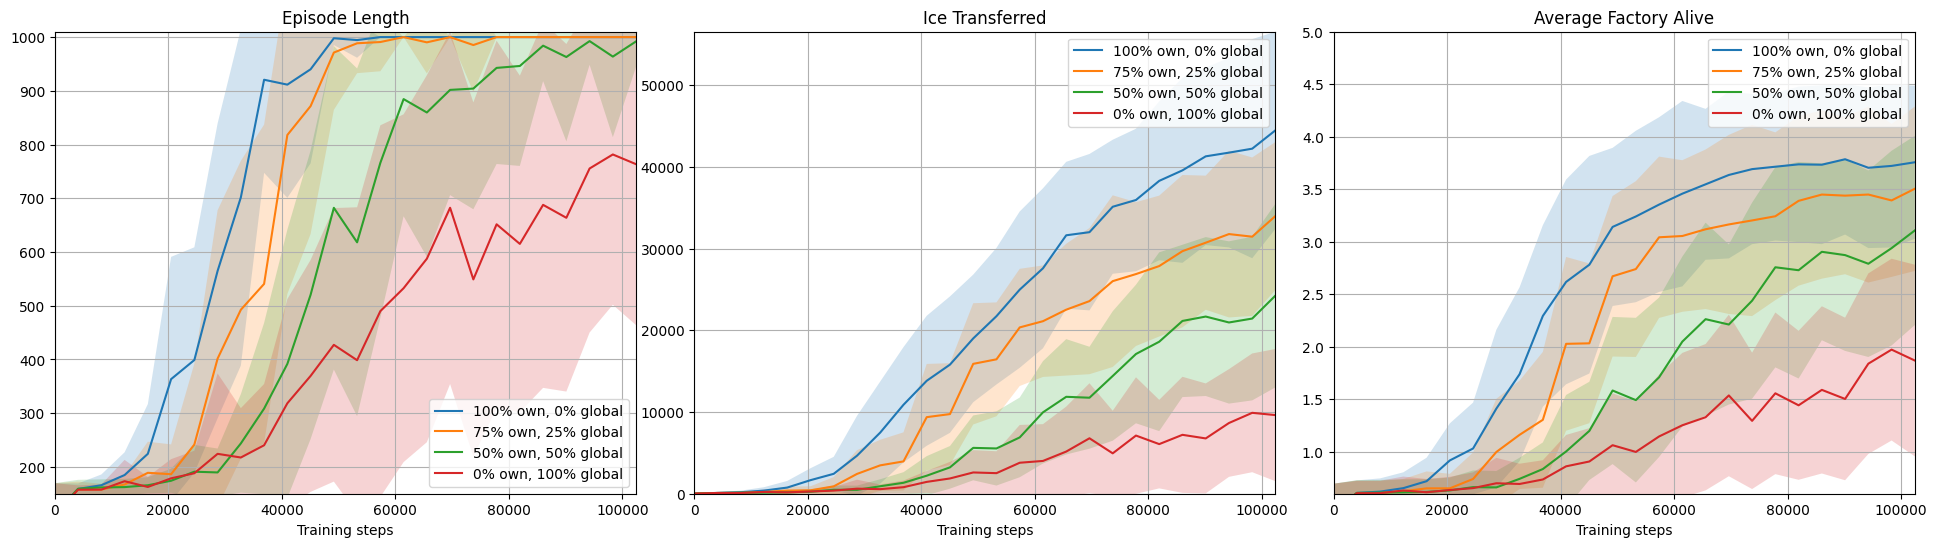
\includegraphics[width=0.95\linewidth]{images/results_hybrid/reward_assignment/combined.png}
    \captionsetup{justification=justified, singlelinecheck=false, width=1\linewidth, labelfont=bf} 
    \caption[]{Plot comparing the performance of different percentages of global and local rewards in terms of the length of the episodes, ice transferred by units, and number of active factories. In addition to the test variants, the global and completely separate trajectory variants are also present. Mixing in global rewards seems to hinder performance.}
    \label{fig:hybrid_results/reward_assignment/combined}
\end{figure}

\begin{table}[ht]
    \footnotesize
    \renewcommand{\arraystretch}{1.2}%
    \begin{tabularx}{\textwidth}{|X|C{2.3cm}|C{2.3cm}|C{2.0cm}|C{2.0cm}|}
        \hline
\multicolumn{1}{|Y|}{\textbf{Group Name}} & \textbf{Final Ice Transferred} & \textbf{Final Episode Length} & \textbf{10\% of Episodes Finished by} & \textbf{95\% of Episodes Finished by} \\
        \hline
100\% own, 0\% global & \textbf{44,472 (12,065)} & \textbf{1,000 (0)} & \textbf{28,672 steps} & \textbf{49,152 steps} \\
75\% own, 25\% global & 33,985 (9,059) & \textbf{1,000 (0)} & \textbf{28,672 steps} & 57,344 steps \\
50\% own, 50\% global & 24,244 (11,238) & 992 (47) & 45,056 steps & 94,208 steps \\
0\% own, 100\% global & 9,614 (8,094) & 763 (300) & 53,248 steps & - \\
        \hline
    \end{tabularx}
    \medskip
    \captionsetup{justification=justified, singlelinecheck=false, width=1\linewidth, labelfont=bf} 
    \caption{Table comparing the performance of different global and local reward percentages. The metrics featured include the amount of ice transferred by units and the length of the episodes in the evaluation phase following the last training cycle. The table also contains the observed environment steps needed until the model reaches the maximum episode length in the specified percentage of evaluation environments. In addition to the test variants, the global and completely separate trajectory variants are also present.}
    \label{tab:hybrid_results/reward_assignment/combined}
\end{table}


\subsection{Comparison with Other Works}
\label{subsec:comparison}

\noindent As previously stated in this section, the training objectives in the experiments demonstrating \textbdd{trajectory separation} (\autoref{sec:trajectory-separation}) were focused on achieving the \textbdd{maximum episode length}, which can be accomplished by keeping at least one factory alive from both players. Factories have a \textbdd{lichen watering} action (\autoref{sec:wincondition}), which is used to determine the winner if both players successfully maintain their factories until the maximum duration of the episode. In the previous experiments, we masked out (\autoref{subsec:actions}) this watering action in order to achieve faster convergence. This decision was made since watering can \textbdd{reduce the potential lifespan of a factory}. Consequently, in order to conduct a comparative analysis between our approach and state-of-the-art solutions, it was necessary to enable lichen watering. As a result, we proceeded to train a \textbdd{slightly different} version of our model. We used trajectory separation without any kind of grouping rule (\autoref{subsec:grouping}) or trajectory sample reduction (\autoref{subsec:tsr}). Given that the other solutions gave rewards for growing lichen, we made adjustments to the reward functions so that the factories received \textbdd{rewards proportional to the number of lichen tiles} present on the board at the end of the episode. Lichen can only be grown on rubbleless tiles; thus, we also rewarded units after \textbdd{clearing away rubble} next to factories and lichen tiles. We measured how long it took for the modified model to learn how to keep the factories alive up to the maximum episode length. The performance of the modified model compared to the original can be observed in \autoref{fig:hybrid_results/lichen_vs_ts/combined} and \autoref{tab:hybrid_results/lichen_vs_ts/combined}. Even though enabling and rewarding the watering action caused a slight decrease in performance, the model still managed to learn how to transport sufficient ice to factories. It also learned how to successfully grow lichen, as can be seen in \autoref{fig:hybrid_results/lichen/combined}.

\begin{figure}[htbp]
    \centering
    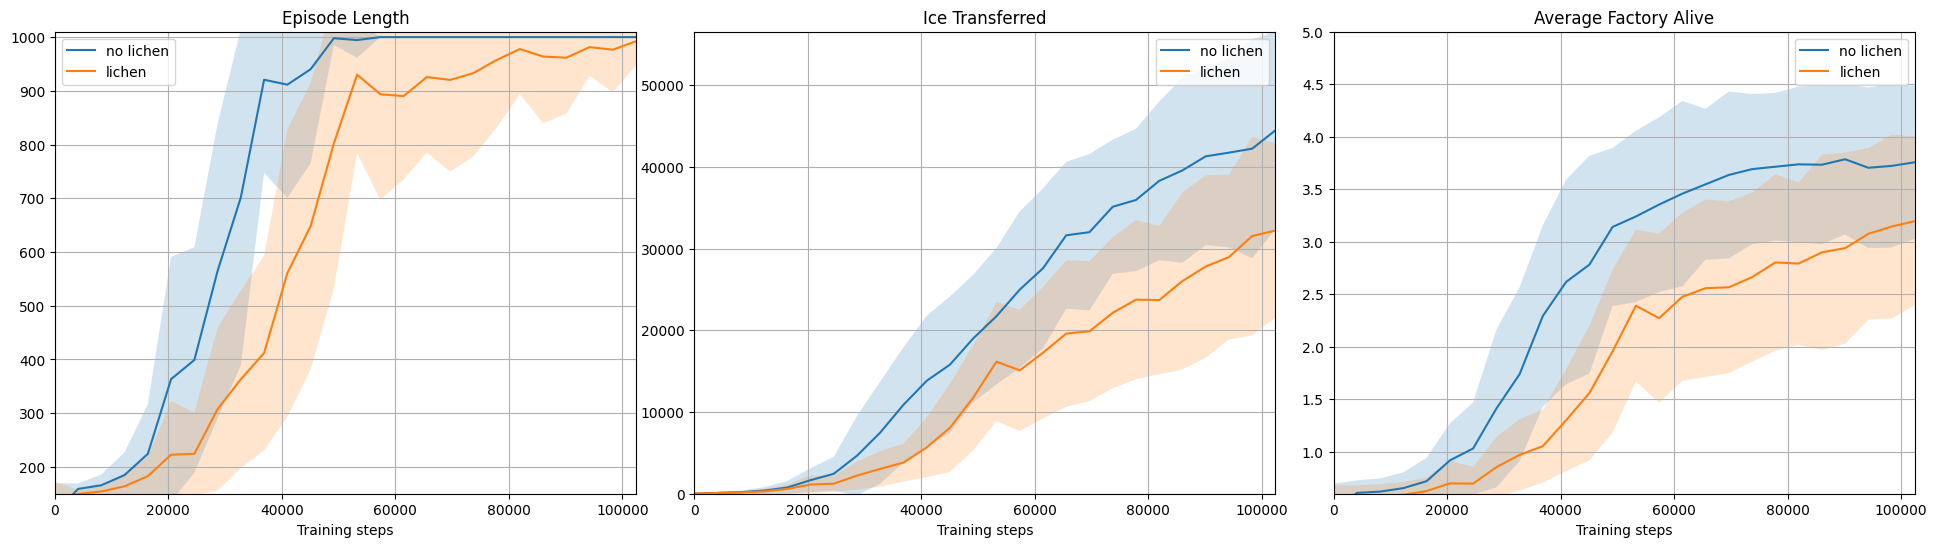
\includegraphics[width=0.95\linewidth]{images/results_hybrid/lichen_vs_ts/combined.png}
    \captionsetup{justification=justified, singlelinecheck=false, width=1\linewidth, labelfont=bf} 
    \caption[]{Plot comparing the performance of the new lichen-enabled model to the original in terms of the length of the episodes, ice transferred by units, and number of active factories. While lichen watering degrades performance, the goal of reaching the maximum episode length is still achieved at the end of the observed step range.}
    \label{fig:hybrid_results/lichen_vs_ts/combined}
\end{figure}

\begin{table}[ht]
    \footnotesize
    \renewcommand{\arraystretch}{1.2}%
    \begin{tabularx}{\textwidth}{|X|C{2.3cm}|C{2.3cm}|C{2.0cm}|C{2.0cm}|}
        \hline
\multicolumn{1}{|Y|}{\textbf{Group Name}} & \textbf{Final Ice Transferred} & \textbf{Final Episode Length} & \textbf{10\% of Episodes Finished by} & \textbf{95\% of Episodes Finished by} \\
        \hline
no lichen & \textbf{44,472 (12,065)} & \textbf{1,000 (0)} & \textbf{28,672 steps} & \textbf{49,152 steps} \\
lichen & 32,199 (10,670) & 992 (45) & 40,960 steps & 102,400 steps \\
        \hline
    \end{tabularx}
    \medskip
    \captionsetup{justification=justified, singlelinecheck=false, width=1\linewidth, labelfont=bf} 
    \caption{Table comparing the performance of the new lichen-enabled model to the original. The metrics featured include the amount of ice transferred by units and the length of the episodes in the evaluation phase following the last training cycle. The table also contains the observed environment steps needed until the model reaches the maximum episode length in the specified percentage of evaluation environments. In addition to the test variants, the global and completely separate trajectory variants are also present. The lichen-enabled variant managed to reach the desired 95\% of completed episodes by the end of the observed step range.}
    \label{tab:hybrid_results/lichen_vs_ts/combined}
\end{table}

\begin{figure}[htbp]
    \centering
    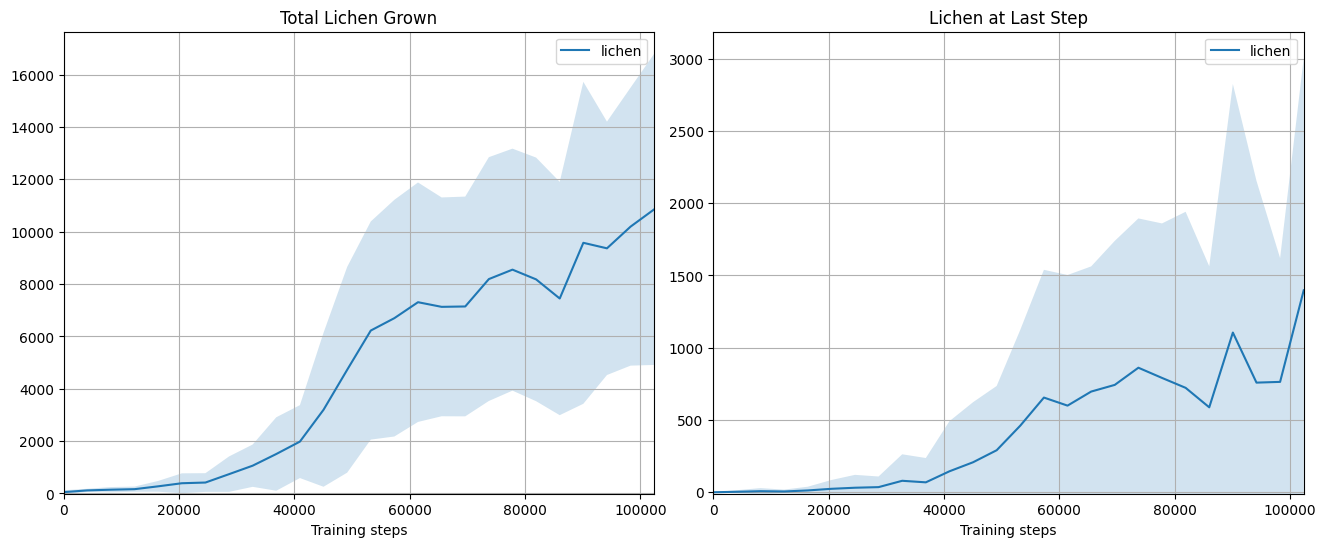
\includegraphics[width=0.95\linewidth]{images/results_hybrid/lichen/combined.png}
    \captionsetup{justification=justified, singlelinecheck=false, width=1\linewidth, labelfont=bf} 
    \caption[]{Plot showcasing the amount of total lichen grown and the amount of lichen at the end of the episodes. In addition to learning how to reach the maximum episode length (\autoref{fig:hybrid_results/lichen_vs_ts/combined}), the agent demonstrated the ability to solve a secondary task, as shown by the ascending lines.}
    \label{fig:hybrid_results/lichen/combined}
\end{figure}

\bigskip

\noindent We wanted to compare our solution to the \textbdd{top-performing submissions} in the Lux AI competition. The basis of our comparison is how long it took for the different models to reach a state where they could \textbdd{keep the factories alive} until the maximum episode length \textbdd{in most environments}. In our case, this goal was 95\% of episodes. Unfortunately, the leaderboards were predominantly controlled by \textbdd{rule-based methods}, resulting in very few RL-based submissions that could be used for a comparative analysis. Many refrained from sharing their work, and in lots of cases where they did share it, their trained models or training metrics were \textbdd{not made publicly available}. The only somewhat reliable source we could find was \textbdd{FLG's submission} (\cite{ferdinand}), which was somewhat similar to the pixel-to-pixel architecture we started with. Their training objective during the initial \textbdd{set-up phase} was comparable to ours, which aimed to teach the agent fundamental aspects of the game, such as gathering resources. The duration of their training in terms of time and steps was outlined; however, we are not sure what their stopping criteria were. Consequently, for the purpose of our comparison, we will assume that the stopping criterion used in the referenced submission was identical to our own. In addition, we included a \textbdd{baseline solution} provided by the competition organizers (\cite{luxai_s2-baseline-source}). The comparison can be seen in \autoref{tab:other-work-comparisons}. Our approach massively outperformed both the baseline and the FLG's submission in every single one of our metrics. We managed to reach the maximum episode length in 95\% of the environments by step 102,400. In comparison, the baseline model required 1.4 million steps to reach the same milestone, while the submission of FLG was trained for 65 million steps. Given that we utilized a larger value for the hyperparameter \textbdd{number of epochs} compared to the baseline, resulting in faster training, we believed it was necessary to account for this difference in our comparison. Having said that, our approach is still 5 times more efficient in terms of weight updates needed. Our approach also yielded significantly reduced model sizes, with a mere 200 thousand trainable parameters, as opposed to 451 thousand and 6.08 million, respectively. We also compared the training times, although it should be noted that the resources used for training the other two solutions remain undisclosed, potentially introducing a bias to the presented values.

\bigskip

% time it took for ours to reach 102k steps:
% 2.143 h
% 2.113 h
% 1.999 h
% avg: 2.085 h

\begin{table}[htbp]
    \footnotesize
    \renewcommand{\arraystretch}{1.2}%
    \begin{threeparttable}
        \begin{tabularx}{\linewidth}{|X|C{2.0cm}|C{2.0cm}|C{2.0cm}|C{2.0cm}|}
            \hline
            \textbf{Solution} & \textbf{Parameters}  & \textbf{Training time} & \textbf{Environment Steps} & \textbf{Training Epochs} \\
            \hline
            Trajectory Separated Hybrid Approach & \textbf{200K} & \textbf{2 hours} & \textbf{102K} & \textbf{250} \\
            Baseline Solution (\cite{luxai_s2-baseline-source}) & 451K & 2 days & 1.4M & 1364 \\
            Best RL Submission (\cite{ferdinand}) & 6.08M & 2 days\tnote{*} & 65M\tnote{*} & ?\tnote{**} \\
            \hline
        \end{tabularx}
        \begin{tablenotes}
            \item[*] exact stopping criterion is not known, only the number of steps the model was trained on and the time of training.
            \item[**] \textbdd{number of epochs} hyperparameter not provided.
        \end{tablenotes}
        \captionsetup{justification=justified, singlelinecheck=false, width=1\linewidth, labelfont=bf} 
        \caption{Table containing the comparison of our work with other implementations. We included the best-performing reinforcement learning submission of the Lux AI competition and a baseline repository provided by the organizers. Our method outperforms both of them in terms of both training time and observed environment steps needed to reach the designated goal. The table also shows a significant difference in model sizes.}
        \label{tab:other-work-comparisons}
    \end{threeparttable}
\end{table}


\subsection{Model Ablation Study}
\label{subsec:ablation}

\noindent Through the utilization of \textbdd{trajectory separation} (\autoref{sec:trajectory-separation}), we achieved a significant acceleration in the training process of our model. However, as previously discussed in \autoref{sec:monolithic-approach} and \autoref{sec:hybrid-approach}, many additional components played an important role in achieving the level of performance described, with \textbdd{certain components being absolutely indispensable}. In this subsection, we performed an ablation study on the key methods employed to demonstrate the various factors that can impact reinforcement learning and the potential pitfalls that can arise.

\subsubsection{Weight Initialization}

\noindent The proper initialization of weights plays a crucial role, particularly in the application of algorithms such as Proximal Policy Optimization (\autoref{sec:ppo}). We have provided an overview of the weight initialization structure of our model in \autoref{subsec:weight-scaling} and will delve into this issue further in \autoref{ch:disc-init-is-all-you-need}. In this study, we aim to illustrate the impact of incorrect initialization on the convergence of our trajectory-separated \textbdd{hybrid} (\autoref{sec:hybrid-approach}) model. The study involved the examination of two components: the weight initialization \textbdd{scaling} in the \textbdd{output layers} and an \textbdd{additional scaling} applied to \textbdd{all the weights} after initialization, referred to as \textbdd{extra scaling}. We tested removing the extra scaling from the hidden layers (\textttdb{"no extra hidden layer scaling"}) as well as from all layers (\textttdb{"no extra scaling"}). We also conducted experiments to evaluate the effects of removing any kind of scaling from the actor output layers (\textttdb{"no actor scaling"}), the critic value output layers (\textttdb{"no value scaling"}), and all output layers (\textttdb{"no scaling"}). As presented in \autoref{fig:hybrid_results/ablation_study/combined_init} and \autoref{tab:hybrid_results/ablation_study/combined_init}, the \textbdd{removal of any} weight initialization component leads to \textbdd{deterioration of performance}. Eliminating all \textbdd{weight-downscaling techniques} renders the model incapable of any kind of learning. The main problem with large weights is their \textbdd{effect on the initial policies}. A network that exhibits a high degree of bias may not assign \textbdd{equal probabilities} to all possible actions, resulting in a decrease in the \textbdd{exploration} of different actions and a slower rate of learning. This biased network can sometimes lead to \textbdd{policy collapse}, as observed with variant \textttdb{"no actor scaling"}. Interestingly, removing the critic value output's scaling causes even larger performance degradation because the early parts of the training must be spent on training the value network to overcome its \textbdd{inherent bias}. As a result, the predicted advantage values, which are essential for the PPO algorithm, will be inaccurate.

\begin{figure}[htbp]
    \centering
    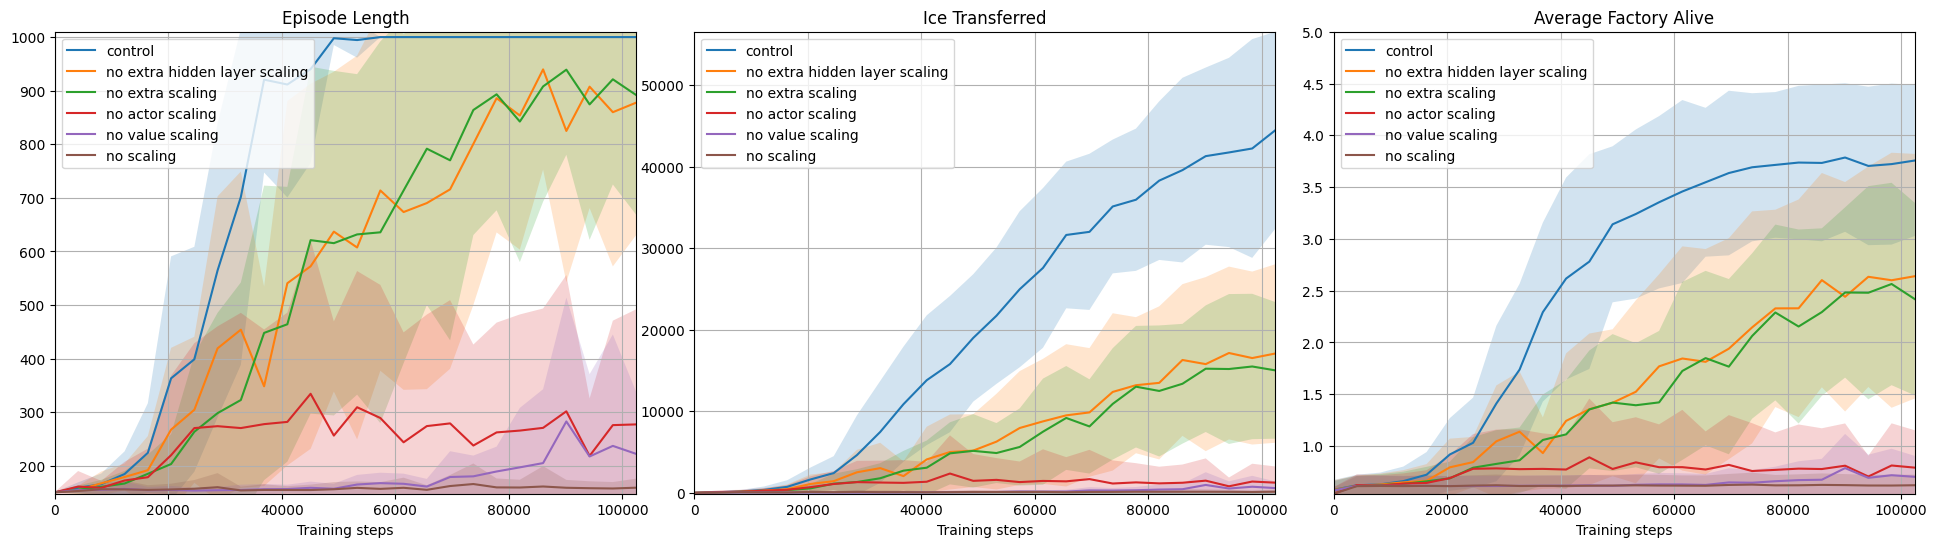
\includegraphics[width=0.95\linewidth]{images/results_hybrid/ablation_study/combined_init.png}
    \captionsetup{justification=justified, singlelinecheck=false, width=1\linewidth, labelfont=bf} 
    \caption[]{Plot showcasing the difference in performance weight magnitudes can cause in terms of the length of the episodes, ice transferred by units, and number of active factories. Removing any kind of weight downscaling caused a significant performance decrease. Not scaling down the weights of the output layer at all makes training impossible for the model.}
    \label{fig:hybrid_results/ablation_study/combined_init}
\end{figure}

\begin{table}[ht]
    \footnotesize
    \renewcommand{\arraystretch}{1.2}%
    \begin{tabularx}{\textwidth}{|X|C{2.3cm}|C{2.3cm}|C{2.0cm}|C{2.0cm}|}
        \hline
\multicolumn{1}{|Y|}{\textbf{Group Name}} & \textbf{Final Ice Transferred} & \textbf{Final Episode Length} & \textbf{10\% of Episodes Finished by} & \textbf{95\% of Episodes Finished by} \\
        \hline
control & \textbf{44,472 (12,065)} & \textbf{1,000 (0)} & \textbf{28,672 steps} & \textbf{49,152 steps} \\
no extra hidden layer scaling & 17,093 (10,944) & 878 (247) & 32,768 steps & - \\
no extra scaling & 15,019 (8,371) & 892 (223) & 36,864 steps & - \\
no actor scaling & 1,255 (1,986) & 277 (215) & 45,056 steps & - \\
no value scaling & 591 (811) & 222 (116) & - & - \\
no scaling & 145 (257) & 159 (17) & - & - \\
        \hline
    \end{tabularx}
    \medskip
    \captionsetup{justification=justified, singlelinecheck=false, width=1\linewidth, labelfont=bf} 
    \caption[]{Table showcasing the difference in performance weight magnitudes can cause. The metrics featured include the amount of ice transferred by units and the length of the episodes in the evaluation phase following the last training cycle. The table also contains the observed environment steps needed until the model reaches the maximum episode length in the specified percentage of evaluation environments. The table clearly shows the decline in performance caused by taking away the weight scalings one by one. None of the studied variants managed to learn how to keep the factories alive until the maximum episode length in most environments.}
    \label{tab:hybrid_results/ablation_study/combined_init}
\end{table}

\subsubsection{Removing Heuristics}

\noindent Our implementation of \textbdd{action masking} (\autoref{subsec:mono-actions}) and \textbdd{factory placement} (\autoref{subsec:heur-bidding-factory}) introduces a great level of \textbdd{heuristics} into the system. Action masking decreases the action space, resulting in faster convergence. Additionally, the strategic placement of factories in close proximity to ice tiles simplifies the environment. Both of these factors play a crucial role, as can be observed in \autoref{fig:hybrid_results/ablation_study/combined_heuristics} and \autoref{tab:hybrid_results/ablation_study/combined_heuristics}. Without the implementation of action masking, the model is presented with an \textbdd{excessive number} of potential combinations in its \textbdd{action space}, leading to an inability to learn an optimal policy. Consequently, there was no significant increase observed in the \textbdd{episode length} metric throughout the entire training period. By setting the factory placement to random, the agents can still learn how to transport ice to factories. However, due to the \textbdd{varying distances} of ice tiles from factories in each episode, the units are \textbdd{unable to learn} how to keep the factories alive within the observed step range.

\begin{figure}[htbp]
    \centering
    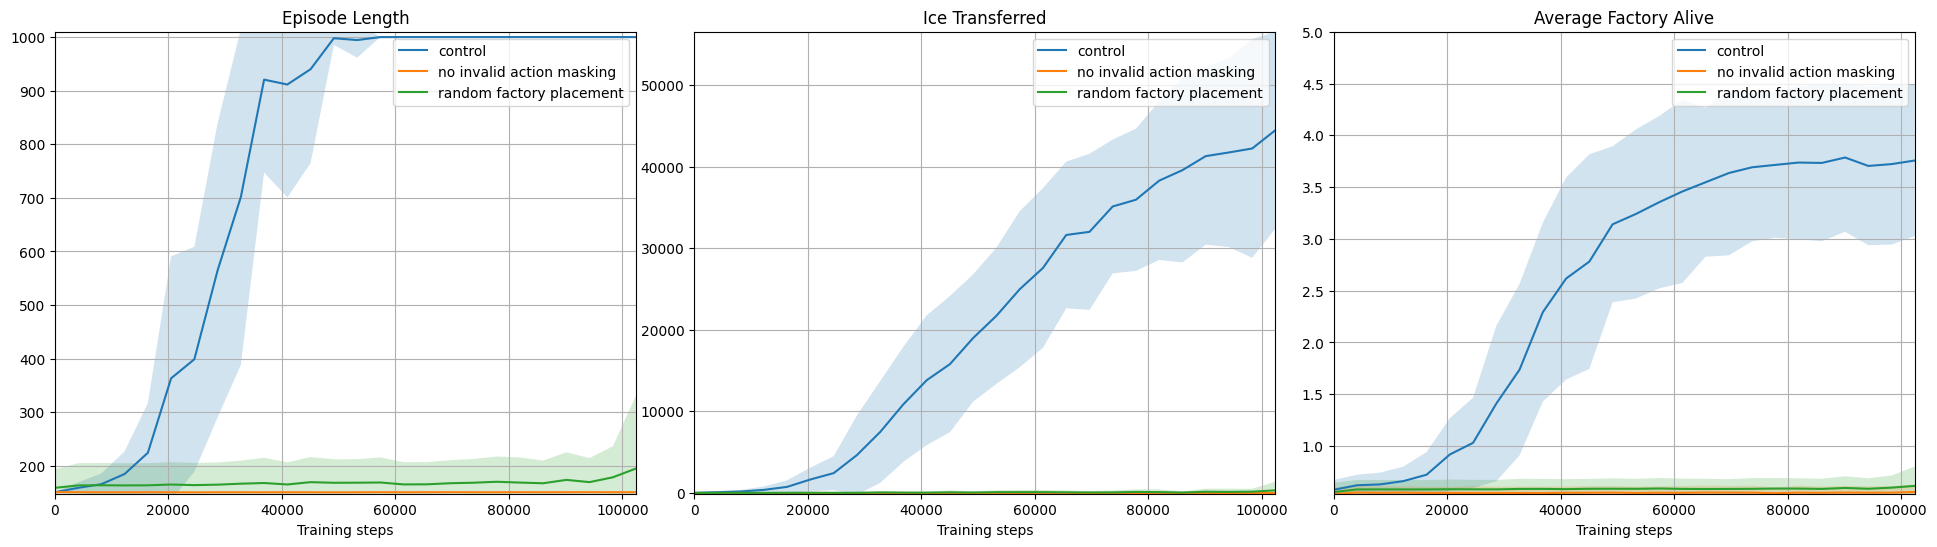
\includegraphics[width=0.95\linewidth]{images/results_hybrid/ablation_study/combined_heuristics.png}
    \captionsetup{justification=justified, singlelinecheck=false, width=1\linewidth, labelfont=bf} 
    \caption[]{Plot showcasing the difference in performance that removing heuristics causes in terms of the length of the episodes, ice transferred by units, and number of active factories. The elimination of action masking renders training infeasible within the specified step range that we have presented. In addition, the placement of factories at random locations introduces complexity to the environment, resulting in a significant decline in performance.}
    \label{fig:hybrid_results/ablation_study/combined_heuristics}
\end{figure}

\begin{table}[ht]
    \footnotesize
    \renewcommand{\arraystretch}{1.2}%
    \begin{tabularx}{\textwidth}{|X|C{2.3cm}|C{2.3cm}|C{2.0cm}|C{2.0cm}|}
        \hline
\multicolumn{1}{|Y|}{\textbf{Group Name}} & \textbf{Final Ice Transferred} & \textbf{Final Episode Length} & \textbf{10\% of Episodes Finished by} & \textbf{95\% of Episodes Finished by} \\
        \hline
control & \textbf{44,472 (12,065)} & \textbf{1,000 (0)} & \textbf{28,672 steps} & \textbf{49,152 steps} \\
no invalid action masking & 0 (0) & 151 (0) & - & - \\
random factory placement & 316 (1,055) & 195 (137) & - & - \\
        \hline
    \end{tabularx}
    \medskip
    \captionsetup{justification=justified, singlelinecheck=false, width=1\linewidth, labelfont=bf} 
    \caption[]{Table showcasing the difference in performance that removing heuristics causes. The metrics featured include the amount of ice transferred by units and the length of the episodes in the evaluation phase following the last training cycle. The table also contains the observed environment steps needed until the model reaches the maximum episode length in the specified percentage of evaluation environments. Without action masking, the units were unable to transfer any ice to factories. Random factory placement still allowed the units to learn that mining and transferring ice are advantageous, but they could not perform said actions optimally.}
    \label{tab:hybrid_results/ablation_study/combined_heuristics}
\end{table}

\subsubsection{Network Regularization}

\noindent In our network, we incorporated two crucial regularization components: \textbdd{batch normalization} (\autoref{subsec:batchnorm}) and \textbdd{spectral norm} (\autoref{subsec:spectralnorm}). In the following experiment, we tested the necessity of employing both regularization methods. As can be seen in \autoref{fig:hybrid_results/ablation_study/combined_net} and \autoref{tab:hybrid_results/ablation_study/combined_net}, it is apparent that the inclusion of \textbdd{some form of regularization is essential}. Removing batch normalization resulted in our model's inability to learn how to reach the maximum episode length within the observed step range. Interestingly, eliminating the spectral norm by itself did not significantly affect performance. Nevertheless, in the \textbdd{absence of batch normalization}, the \textbdd{performance deteriorated} even further when the spectral norm was removed. This observation suggests that the simultaneous use of both regularization methods may not be necessary. However, including \textbdd{at least one of them is crucial}, preferably batch normalization.

\begin{figure}[htbp]
    \centering
    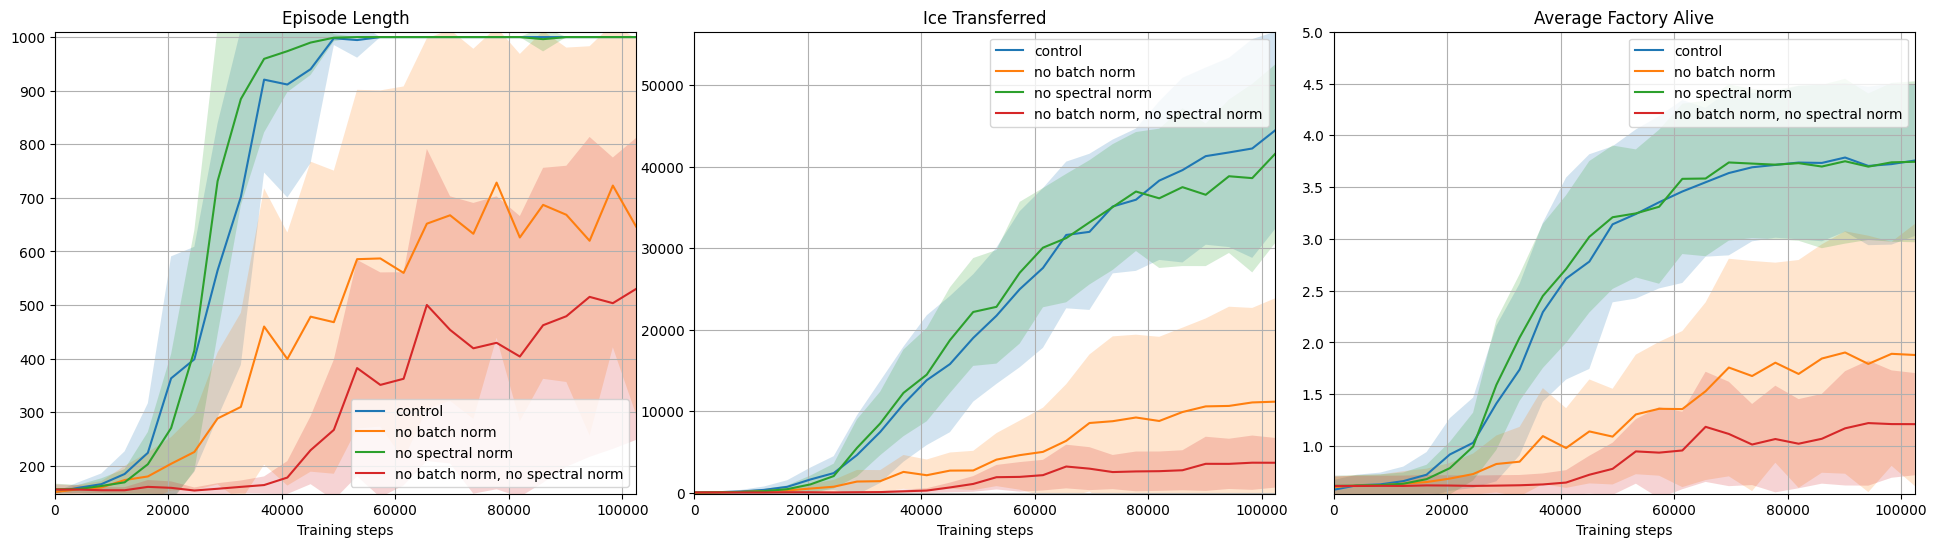
\includegraphics[width=0.95\linewidth]{images/results_hybrid/ablation_study/combined_net.png}
    \captionsetup{justification=justified, singlelinecheck=false, width=1\linewidth, labelfont=bf} 
    \caption[]{Plot showcasing the difference in performance that removing regularization from our network causes in terms of the length of the episodes, ice transferred by units, and number of active factories. It is clearly visible that batch normalization is the most important regularization component. However, if there is no batch normalization utilized in the network, the presence of spectral norm can help mitigate the need for regularization. Removing batch normalization appears to also cause high variance in the observed metrics.}
    \label{fig:hybrid_results/ablation_study/combined_net}
\end{figure}

\begin{table}[ht]
    \footnotesize
    \renewcommand{\arraystretch}{1.2}%
    \begin{tabularx}{\textwidth}{|X|C{2.3cm}|C{2.3cm}|C{2.0cm}|C{2.0cm}|}
        \hline
\multicolumn{1}{|Y|}{\textbf{Group Name}} & \textbf{Final Ice Transferred} & \textbf{Final Episode Length} & \textbf{10\% of Episodes Finished by} & \textbf{95\% of Episodes Finished by} \\
        \hline
control & \textbf{44,472 (12,065)} & \textbf{1,000 (0)} & \textbf{28,672 steps} & 49,152 steps \\
no batch norm & 11,184 (12,688) & 646 (351) & 53,248 steps & - \\
no spectral norm & 41,611 (10,938) & \textbf{1,000 (0)} & \textbf{28,672 steps} & \textbf{45,056 steps} \\
no batch norm, no spectral norm & 3,696 (3,039) & 530 (282) & 65,536 steps & - \\
        \hline
    \end{tabularx}
    \medskip
    \captionsetup{justification=justified, singlelinecheck=false, width=1\linewidth, labelfont=bf} 
    \caption[]{Table showcasing the difference in performance that removing regularization from our network causes. The metrics featured include the amount of ice transferred by units and the length of the episodes in the evaluation phase following the last training cycle. The table also contains the observed environment steps needed until the model reaches the maximum episode length in the specified percentage of evaluation environments. Removing batch normalization decreases the model's performance significantly, making it unable to learn how to reach the maximum episode length in all environments. Removing spectral norms further degrades performance.}
    \label{tab:hybrid_results/ablation_study/combined_net}
\end{table}
